% Dokumentenklasse scrreprt                             %
\documentclass[11pt, rgb]{scrreprt}
\RequirePackage{etex} % is required to prevent stuff
\usepackage{csquotes} % Bibtex and language stuff

\usepackage{rotating}
\usepackage{lmodern}

\hyphenation{Bei-stand}
\hyphenation{Su-pra-strom}
\hyphenation{pro-gress}

% weniger Farbe dann Addons
% \usepackage{corporatedesign/themeKonstanzXelatexAddOn} % XeLaTeX mit Schriftart Arial, VOR dem Standardpaket importieren
\usepackage{corporatedesign/themeKonstanz} % Muss immer verwendet werden (Standardpaket)
% \usepackage{corporatedesign/themeKonstanzStyleAddOn} % Style Add-On für andere Überschriften, NACH dem Standardpaket importieren

% \setstocksize{297mm}{210mm} % or format a4
\format{a4} %A4, vllt. A5?

% Dokumentinformationen        
\date{\today}
\year{2021}
\author{Oliver Irtenkauf}
%\title{\selectfontsize{32pt}\flushright\markieren{Electronic transport in}{superconducting ferromagnetic}{hetero-structures}{under microwave irradiation}}
\title{Electronic transport in superconducting ferromagnetic hetero-structures under microwave irradiation}
\title{Broadband ferromagnetic resonance measurements\\on thin cobalt films at low temperatures}
\subtitle{Master's Thesis}
\unisection{Faculty of Science}
\department{Department of Physics}
\supervisorOne{Prof. Dr. Elke Scheer}
\supervisorTwo{Prof. Dr Angelo Di Bernardo}

% Kopf und Fusszeile           
\headFoot{9}

% use bibliography.bib
\usepackage[backend=biber, sorting=none, maxbibnames=99]{biblatex}
\addbibresource{bibliography.bib}

% For blank page
\usepackage{afterpage}
\newcommand\blankpage{
    \null
    \thispagestyle{empty}
    \addtocounter{page}{-1}
    \newpage
    }

% for formular
\usepackage{amsmath}

% blindtext
\usepackage{subcaption}\usepackage{blindtext}

%\renewcommand{\thesubfigure}{\roman{subfigure}}

% import inkscape
\usepackage{import}
\usepackage{textcomp}  %\textmu
% \graphicspath{setup/}

% renew vec
\usepackage{amsmath}
\renewcommand{\vec}[1]{\mathbf{#1}}

\newcommand{\ima}[0]{\overset{\hspace{0.9mm}\text{\scalebox{0.7}{$\circ$}}}{\imath}}

% for python code
\usepackage{listings}
\definecolor{codegreen}{rgb}{0,0.6,0}
\definecolor{codegray}{rgb}{0.5,0.5,0.5}
\definecolor{codepurple}{rgb}{0.58,0,0.82}
\definecolor{backcolour}{rgb}{0.95,0.95,0.95}
\lstdefinestyle{mystyle}{
    backgroundcolor=\color{backcolour},   
    commentstyle=\color{seeblau100},
    keywordstyle=\color{antiseeblau100},
    numberstyle=\tiny\color{codegray},
    stringstyle=\color{seeblau65},
    basicstyle=\ttfamily\tiny,
    breakatwhitespace=false,         
    breaklines=true,                 
    captionpos=b,                    
    keepspaces=true,                 
    numbers=left,                    
    numbersep=5pt,                  
    showspaces=false,                
    showstringspaces=false,
    showtabs=false,                  
    tabsize=2
}
\lstset{style=mystyle}
\usepackage{multicol}
\setlength{\columnsep}{30pt}
\usepackage{pdflscape}
\interfootnotelinepenalty=10000
%%%%%%%%%%%%%%%%%%%%%%%%%%%%%%%%%%%%%%%%%%%%%%%%%%%%%%%%%
% Begin of Document                                     %
%%%%%%%%%%%%%%%%%%%%%%%%%%%%%%%%%%%%%%%%%%%%%%%%%%%%%%%%%


\begin{document}
%\afterpage{\blankpage}
\thesistitlepage[language=english]{Master's Thesis}

% \afterpage{\blankpage}
% % \unititlepage[graphic=graphics/Snap-3227.jpg]{}
% \unititlepagey[graphic=corporatedesign/title graphics/rose1.jpg]{}
% \afterpage{\blankpage}
% \unititlepage[graphic=corporatedesign/title graphics/rose1.jpg]{}

\pagenumbering{Roman}

% Introduction
% Previous or relevant references
% The goal of the project
% How that goal was met
% Key results
% What makes your results unique or noteworthy

% Through ferromagnetic resonance excitation, a long-range spin triplet supercurrent can flow through a ferromagnetic barrier, according to the theoretical prediction of Hikino et al [1, 2]. For electronic transport measurements through a superconductor-ferromagnet-superconductor contact, the dimension, such as the thickness, of the ferromagnet is crucial. Therefore, Co films as thin as 3 nm were prepared by electron beam evaporation with a co-planar waveguide on top. Transmission measurements were performed at cryogenic temperatures using an in-plane magnet and a broadband vector network analyzer.
%A quantitative correlation between ferromagnetic resonance frequency and applied magnetic field could be established.

% Entsprechend der Theorie nach Hikino et al \cite{Hikino2007,Hikino_2011} kann durch ferromagnetische Resonanzanregung ein langreichweitiger Spin-Triplett-Suprastrom durch eine ferromagnetische Barriere flie\ss en. Für elektronische Transportmessungen durch einen Supraleiter-Ferromagnet-Supraleiter-Kontakt sind Abmessungen wie die Dicke des Ferromagneten entscheidend. Daher wurden Kobaltfilme mit einer Dicke von $3\,$nm durch Elektronenstrahlverdampfung mit einem koplanaren Wellenleiter auf der Oberseite hergestellt. Transmissionsmessungen wurden bei kryogenen Temperaturen mit einem parallelen Magnetfeld und einem breitbandigen Vektor-Netzwerkanalysator durchgeführt.
% Es konnte eine quantitative Korrelation zwischen der ferromagnetischen Resonanzfrequenz und dem angelegten Magnetfeld hergestellt werden.


%\noindent\begin{minipage}[b][.49\textheight]{\textwidth}
\chapter*{Zusammenfassung}
Es ist bekannt, dass durch ferromagnetische Resonanz (FMR) Anregungen ein reiner Spinstrom aus einem präzidierenden Ferromagneten (F) in ein normales Metall (N) eingekoppelt werden kann. Dieser Spinstrom kann in spintronischen Bauelementen zur Kodierung und Verarbeitung digitaler Informationen genutzt werden.

Ähnlich wie im Fall von F/N-Systemen wurde kürzlich vorgeschlagen, dass ein vollständig spinpolarisierter (Spin-Triplett) supraleitenden Strom (Suprastrom) auch in Supraleiter/Ferromagneten (S/F) Systemen erzeugt werden kann und somit zur Nutzung von Spintronik-Operationen mit geringen Energieverlusten im supraleitenden Regime eingesetzt werden kann. Im Gegensatz zu konventionellen Supraströmen, die aus antiparallel ausgerichteten (Spin-Singulett) Cooper-Paaren von Elektronen bestehen, sind Spin-Triplett Supraströme nicht nur spinpolarisiert, sondern auch langreichweitig innerhalb eines F. Folglich könnte man durch Realisierung eines S/F/S-Josephson-Bauelements und Anregung einer FMR der F-Schicht von einem Zustand, in dem kein Transport zwischen den beiden S-Schichten stattfindet (aufgrund des schnellen Abklingens des Spin-Singlet Suprastroms in F), zu einem Zustand wechseln, in dem die beiden S-Schichten stattdessen über einen Spin-Triplett Suprastrom gekoppelt sind, der durch die FMR-Anregung von F ausgelöst wird. Um solche supraleitenden Bauelemente zu realisieren, die über FMR-Anregung geschaltet werden können, scheint es entscheidend zu sein, das FMR-Signal von ultradünnen F-Schichten auslösen und detektieren zu können.

Basierend auf diesen Beweggründen wird in dieser Arbeit ein Aufbau zur hochempfindlichen Messung des FMR-Signals von ultradünnen Co (F)-Schichten (bis zu $\approx3\,$nm Dicke) diskutiert. Die ultradünnen Co-Schichten werden durch Elektronenstrahlverdampfung erzeugt, gefolgt von der Herstellung eines koplanaren Wellenleiters darauf. Mikrowellentransmissionsmessungen werden bei niedrigen Temperaturen unter Verwendung eines in der Ebene liegenden Magnetfeldes und eines breitbandigen Vektornetzwerkanalysators durchgeführt. Eine quantitative Beziehung zwischen der FMR Frequenz und dem angelegten Magnetfeld wird hergestellt. Die Funktionsweise des Aufbaus einschlie\ss lich seiner Optimierung in Bezug auf die Rauschunterdrückung des FMR-Signals wird diskutiert. Die erzielten Ergebnisse zeigen die Eignung des Aufbaus für die Charakterisierung der Transporteigenschaften von S/F/S-Bauteilen unter FMR-Anregung.

%\end{minipage}
%https://www.nature.com/articles/s41563-018-0058-9.pdf

%\noindent\begin{minipage}[.49\textheight]{\textwidth}
\chapter*{Abstract}
It is well-established, that through ferromagnetic resonance (FMR) excitation a pure spin current can be injected from a precessing ferromagnet (F) into a normal metal (N) material. This spin current can be used in spintronic devices for the encoding and processing of digital information.

Similar to the case of F/N systems, very recently it has been suggested that a fully spin-polarized (spin-triplet) superconducting current (supercurrent) can be generated also in superconductor/ferromagnet (S/F) systems, and therefore applied to perform spintronics operations with low energy dissipation in the superconducting regime.	Unlike conventional supercurrents that consist of antiparallel-aligned (spin-singlet) Cooper pairs of electrons, spin-triplet supercurrents are not only spin-polarized but also long-ranged inside a F. As a result, by realizing a S/F/S Josephson device and exciting a FMR of the F layer, one could switch from a state where no transport occurs between the two S layers (due to the quick decay of the spin-singlet supercurrent in F) to a state where the two S layers are instead coupled via a spin-triplet supercurrent triggered via the FMR excitation of F. To realize such superconducting devices, which can be switched via FMR excitation, it appears crucial to be able to trigger and detect the FMR signal from ultrathin F layers.

Based on these motivations, in this thesis a setup for high-sensitivity measurement of the FMR signal from ultrathin Co (F) thin films (down to $\approx3\,$nm in thickness) is discussed. The ultrathin Co thin films are grown by electron beam evaporation followed by the fabrication of a co-planar waveguide on top of them. Microwave transmission measurements are performed at low temperatures, using an in-plane magnetic field and a broadband vector network analyzer. A quantitative relation between FMR frequency and applied magnetic field is derived. The performance of the setup including its optimization in terms of noise reduction of the FMR signal is discussed. The results obtained demonstrate the suitability of the setup for the characterization of the transport properties of S/F/S devices under FMR excitation.
%\end{minipage}



% inspirational quote
\newpage\null\vfill\begin{center}
{\selectfontsize{14pt}\underline{\textbf{Kleines Statement}
\footnote{Kristiane Allert-Wybranietz ($^*$1955)}}}%, Trotz Alledem
\vspace{0.8cm}\\Hineinflie\ss en\\in die Formen,\\die sich stellen.\\
Sich aber nicht\\formen lassen\\und auf keinen Fall\\erhärten.\\
\vspace{2mm} Das wäre\\Leben\\für mich.\\\vspace{6cm}\ \\
\end{center}\vfill

\tableofcontents




\clearpage 
\pagenumbering{arabic}

%%%%%%%%%%%%%%%%%%%%%%%%%%%%%%%%%%%%%%%%%%%%%%%%%%%%%%%%%
% Body of Document                                      %
%%%%%%%%%%%%%%%%%%%%%%%%%%%%%%%%%%%%%%%%%%%%%%%%%%%%%%%%%
\chapter{Introduction}

The field of spintronics utilizes the targeted manipulation of spin currents. The goal is to build devices with high energy efficiency either for large computer clusters or for quantum mechanical applications. The physical concept of superconductivity comes in handy at this point, but raises the question of how to specifically manipulate the spin of the superconducting current (supercurrent). As a consequence, the interface between superconductor (S) and ferromagnet (F) is of great interest.

When considering conventional superconductivity, according to Bardeen, Cooper \& {Schrieffer\,\,\cite{BCS1957}}, Cooper pairs consist of two electrons with opposite momentum and spin. Due to the total spin $S=0$ rapid dephasing of the Cooper pair occurs in ferromagnets within only a few nanometers and therefore long-range supercurrents are forbidden within them.

However, according to Fulde, Ferrel, Larkin \& Ovchinnikov \cite{FF1964, LO1969} Cooper pairs can come in triplet states with total spin $S=1$. Antiparallel spin pairs ($S_z=0$) oscillate in the external magnetic field between antiparallel singlet and triplet states during their rapid dephasing. An external magnetic field has no pair-breaking effect on parallel triplet pairs ($S_z=\pm 1$), resulting in much slower dephasing, which is why they are also called long-range spin triplets. A schematic of the different Cooper pairs is shown in Figure \ref{fig:intro_triplet}. As a consequence, a ferromagnet of sufficient size can be used as a spin polarizer for supercurrents if long-range spin triplets are present. 

Besides the static excitation of spin-triplet pairs by complex interlayers  \cite{Keitzer2006, Robinson2010, Kalcheim2014, eschrig2015}, this should also be possible in a dynamical system by magnon absorption. This was predicted by Hikino et al. \cite{Hikino2007,Hikino_2011} and provided with evidence by Jeon et al. \cite{Jeon2018}. Subsequently, this means that a long-range spin current can be induced through a S/F/S Josephson contact by microwave irradiation at the frequency of ferromagnetic resonance (FMR) without the need for special interface preparation. 

In summary, I am interested in the ferromagnetic properties of such an S/F/S contact. In this thesis I share with you my results on resolving the FMR of thin Co films with broadband measurements at different in-plane magnetic fields and cryogenic temperatures.

First, I will recall magnetization dynamics theory that leads to the description of FMR.  Then, I will present the samples and the setups used in my experiments. Next, I will present my more technical findings related to encountered technical problems during my measurements. Finally, I will also discuss the magnetization properties obtained by FMR measurements.

\begin{figure}[b]
    \centering
    \vspace{-2mm}
    \import{theory/triplet}{triplet3.pdf_tex}
    \vspace{-2mm}
    \caption[Scheme of singlet and triplet Cooper pair states]{Schematic of the singlet ($S=0$) and triplet ($S=1$) Cooper pair states. The precession cones of the spins in the externally applied magnetic field along $z$ are shown in \textbf{\color[rgb]{0.5276,0.5276,0.5276}grey} and the two single spins in \textbf{\color{antiseeblau100}magenta} and \textbf{\color{seeblau100}blue}. Depending on their orientation, the total spin of a Cooper pair can have a finite $S_z=\pm 1$ or vanishing $z$-component $S_z=0$. \cite{eschrig2015}}
    \label{fig:intro_triplet}
\end{figure}
\chapter{Theory}
In this Chapter in order to understand the ferromagnetic resonance (FMR) technique I want to recall some basic concepts of magneto dynamics. Furthermore, I also want to give a short excursion into the coherence lengths of singlet and triplet Cooper pairs, since they are needed to define my samples dimensions reasonably. Finally, I want to present you the current state of the art, in the field of FMR measurements on thin ferromagnetic films.

%%%%%%%%%%%%%%%%%%%%%%%%%%%%%%%%%%%%%%%%%%%%%%%%%%%%%%%%%%%%%%%%%%%%%%%%%%%%%%%%%%%%%%%%%%%%%
\section{Landau-Lifshitz-Gilbert Model}
The dynamic magnetic properties of a ferromagnet can be described by damped precessional motion of the exchange-coupled magnetic moments.
If the externally applied magnetic fields and excitation energies are significantly smaller than the exchange coupling energy, we can describe the whole ferromagnet as a macroscopic magnetic spin by the Landau-Lifshitz-Gilbert (LLG) model. \cite{LANDAU199251, Gilbert2004}

The LLG differential equation for the magnetization $\vec{M}$ is given by
\begin{align}
\frac{\text{d}\vec{M}}{\text{d}t}=\underbrace{-\left|\gamma\right| \left(\vec{M}\times \mu_0 \vec{H}_\text{eff}\right)}_{(1)}
+\underbrace{\frac{\alpha}{\left|\vec{M}\right|}\left( \vec{M}\times \frac{\text{d}\vec{M}}{\text{d}t}\right)}_{(2)}\,,\label{formula:LLG}
\end{align}
where $\gamma$ is the gyro-magnetic ratio, $\alpha$ is the Gilbert damping parameter and $\mu_0$ is the vacuum permeability. The effective magnetic field is given by $\vec{H}_\text{eff}=\vec{H}+\vec{H}_\text{ani}$, with $\vec{H}$ being the externally applied magnetic field and $\vec{H}_\text{ani}$ the anisotropy field. 

For better understanding of the LLG model, we first neglect the Gilbert damping term (2) in equation \ref{formula:LLG}. With this neglection the LLG equation simply describes the precession of the magnetization $\vec{M}$ around the effective field $\vec{H}_\text{eff}$. Here the gyro-magnetic ratio is given by $\gamma_\text{e}=\frac{g_\text{e}\mu_\text{B}}{\hbar}=\frac{g_\text{e}q_\text{e}}{2m_\text{e}}$, where $\hbar$ is the reduced Planck constant, $\mu_\text{B}$ the Bohr magneton, $g_\text{e}$, $q_\text{e}$ and $m_\text{e}$ describe the $g$-factor, charge and mass of the free electron respectively. Since the magnetism in ferromagnets, especially in Co, is caused by the electron spins, we can assume a $g$-factor $g\approx 2$ and thus a gyromgnetic ratio of $\frac{\gamma}{2\pi}=28.025$\,GHzT$^{-1}$.
The precession frequency $\omega_\text{res}$ is given by
\begin{align}
    \omega_\text{res}=\gamma\mu_0|\vec{H}_\text{eff}|\,,
\end{align}
resulting in typical resonance frequencies $\omega_\text{res}/2\pi$ in the GHz range, for a few Tesla of applied external magnetic field.

Now we consider the phenomenological Gilbert term (2) from equation \ref{formula:LLG}. After the displacement of $\vec{M}$, it precesses in a spiral trajectory back to its equilibrium position. This relaxation is due to the scattering of phonons and magnons and can be characterised by the relaxation rate $\kappa$. This rate is related to the frequency linewidth by $\Delta\omega=\frac{1}{2\kappa}$, where the linewidth $\Delta\omega$ is usually defined as full width at half maximum (FWHM) and $\kappa$ as the inverse of the half width at half maximum (HWHM).
Now the linewidth $\Delta\omega$ is  connected to the Gilbert parameter $\alpha$ by
\begin{align}
    \Delta\omega=2\alpha\omega_\text{res}+\Delta\omega_0\,.
\end{align}
The inhomogeneous broadening $\Delta\omega_0$ is caused by magnetic inhomogeneities or surface effects. \cite{Beaujour2009}

In order to solve the LLG differential equation \ref{formula:LLG} we will neglect for now the field anisotropy $\vec{H}_\text{ani}=0$. To this end we split the applied magnetic field $\vec{H}$ and magnetization $\vec{M}$ into static ($\vec{H}_0, \vec{M}_0$) and dynamic ($\vec{h}, \vec{m}$) components.
\begin{align}
    \vec{H}&=\vec{H}_0+\vec{h}(t)\label{formula:LLG_field}\\
    \vec{M}&=\vec{M}_0+\vec{m}(t)
\end{align}
Next we assume a static magnetic field in $z$-direction and a dynamic field in $x$- and $y$-direction $\vec{H}=\left(h_x(t),h_y(t),H_0\right)$. If the dynamic magnetic field is much smaller than the static magnetic field, we can also write for the magnetization $\vec{M}=\left(m_x(t),m_y(t),M_0\right)$. Here is $M_0$ the absolute static magnetization. The solution is given by $\vec{m}=\boldsymbol{\chi}\vec{h}$. The two-dimensional Polder tensor $\boldsymbol{\chi}$ is given by
\begin{align}
    \boldsymbol{\chi}=
    \left(
    \begin{array}{cc}
        \chi_{11} & i\chi_{12} \\
        -i\chi_{12} & \chi_{22}
    \end{array}
    \right)\,.
\end{align}
\cite{gurevich1996magnetization}

Since we neglect magnetic field anisotropy, the diagonal elements are the same $\chi=\chi_{11}=\chi_{22}$. Further, we neglect every higher damping therm $\mathcal{O}(\alpha^2)$, in order to get the linear response of a ferromagnet in an external field. Finally, the Polder susceptibility is then given by
\begin{align}
    \chi(\omega,H_0)=\frac{\omega_M\left(\gamma\mu_0H_0-i\Delta\omega\right)}
    {\left( \omega_\text{res}(H_0)\right)^2-\omega^2-i\omega\Delta\omega}\,. \label{eq:chi}
\end{align}
Here is the magnetization frequency  $\omega_M=\gamma\mu_0 M_0$ and the resonance frequency $\omega_\text{res}$. In Figure \ref{fig:theo_chi}, you can see the qualitative behaviour of the Polder susceptibility $\chi(\omega)$ around the resonance frequency $\omega_\text{res}$. \cite{schneider2007, Kalarickal2006}
\begin{figure}
     \centering
     \begin{subfigure}[b]{.33\textwidth}
         \centering
    \import{theory/chi}{chi.pgf}
         \caption{Complex susceptibility $\chi(\omega)$}
         \label{fig:theo_chi}
     \end{subfigure}
     \hfill
     \begin{subfigure}[b]{.6\textwidth}
         \centering
    \import{theory/chi}{wres.pgf}
         \caption{Resonance frequency $\omega_\text{res}/2\pi(\mu_0H_0)$}
         \label{fig:theo_wres}
     \end{subfigure}
        \caption[Schematic of the Polder susceptibility and simulation of the resonance frequency]{\textbf{(a)} Schematic of the complex Polder susceptibility $\chi(\omega)$ in arbitrary units, according to equation \ref{eq:chi}. The maximum of the real part (\textbf{\color{seeblau100}blue}) and the zero crossing of the imaginary part (\textbf{\color{antiseeblau100}magenta}) are marking the resonance frequency $\omega_\text{res}$. The FWHM of the real part and the distance between the minimum and maximum of the imaginary part is marking the line width $\color[rgb]{0.520000,0.520000,0.520000}\pmb{\Delta}\boldsymbol{\omega}$.
        \\\textbf{(b)} Simulation of the ferromagnetic resonance frequency $\omega_\text{res}/2\pi(\mu_0H_0)$, according to equation \ref{formula:kittel1}-\ref{formula:kittel3}. Shown are the curves for the three most common shape anisotropies, that of a sphere (\textbf{\color[rgb]{0.520000,0.520000,0.520000}grey}), an in-plane (\textbf{\color{seeblau100}blue}) or an out-of-plane (\textbf{\color{antiseeblau100}magenta}) magnetized thin film. Parameters: $M_0=8\,$kOe \& $\gamma=28.025\,$GHzT$^{-1}$}
        \label{fig:theo_chi_wres}
\end{figure}

%%%%%%%%%%%%%%%%%%%%%%%%%%%%%%%%%%%%%%%%%%%%%%%%%%%%%%%%%%%%%%%%%%%%%%%%%%%%%%%%%%%%%%%%%%%%%
\newpage
\section{Kittel Formula}\label{sec:theo_Kittel}
Most macroscopic ferromagnets have two opposite favorable directions in which they are most easily magnetized. The so-called easy-axis, which is parallel to the two directions, can be of different origin. In the following simplest case the sample shape anisotropy is treated. Here the magnetic field $\vec{H}$ can be written as follows:
\begin{align}
    \vec{H}=\vec{H}_0+\vec{H}_\text{demag}+\vec{h}(t)\,.
\end{align}

The demagnetization field is given by $\vec{H}_\text{demag}=\vec{N}\cdot\vec{M}$, where the spatially independent demagnetization tensor $\vec{N}$ is in diagonal form, with elements $N_{x,y,z}$.
The resonance frequency can be written as
\begin{align}
    \omega_\text{res}=\gamma\mu_0\sqrt{\left(H_0+(N_y-N_z)M_0\right)\left(H_0+(N_x-N_z)M_0\right)}\,,\label{formula:kittel}
\end{align}
if the applied magnetic field is in the direction of the $z$-axis.

These demagnetisation factors $N_{x,y,z}$ are strongly dependent on the sample geometry. The three most common geometries are discussed below. 
\begin{enumerate}
    \item spherical geometry ($N_{x,y,z}=1/3$).
    \begin{align}
        \omega_\text{res}^\circ=\gamma\mu_0H_0\label{formula:kittel1}
    \end{align}
    \item thin out-of-plane magnetized film ($N_{x,y}=0, N_z=1$).
    \begin{align}
        \omega_\text{res}^\perp=\gamma\mu_0(H_0-M_0)\label{formula:kittel2}
    \end{align}
    \item thin in-plane magnetized film ($N_{x,z}=0, N_y=1$).
    \begin{align}
        \omega_\text{res}^\parallel=\gamma\mu_0\sqrt{H_0(H_0+M_0)}\label{formula:kittel3}
    \end{align}
\end{enumerate}
The ferromagnetic resonance frequencies are simulated in Figure \ref{fig:theo_wres}. 

If there are no other anisotropies than shape anisotropy, $M_0$ is replaced by the saturation magnetization $M_\text{s}$. \cite{kittel1996}

If uniaxial field anisotropy is present, $H_0$ is replaced by $H_\text{eff}=H_0+H_\text{ani}$. For thin in-plane magnetized films, the uniaxial field anisotropy is typically on the order of a few mT. \cite{Kalarickal2006}

At this point, it should be noted that we do not know with certainty whether the easy-axis in thin Co films is in-plane, because out-of-plane easy-axis is also possible. With a suitable substrate, such as Au or Pt, single-digit monolayers of Co, and a suitable cap, such as Au or Ag, out-of-plane magnetization of Co may be present. In addition, there are studies of Co films as thin as $40\,$nm that both at normal and oblique incidence of atomic current during electron beam evaporation Co always exhibit in-plane easy-axis.
At this point, I suspect that Co exhibits robust in-plane magnetization and only shows out-of-plane magnetization under very special conditions. \cite{Su2003, McGee1993, Ujfalussy1996, SZUNYOGH1997}

Furthermore, it should be considered that superconductors, such as aluminum, have a critical magnetic field of only a few mT. Only for very thin films, in the single-digit nanometer range, aluminum can achieve an in-plane critical field in the Tesla range. To use a finite ferromagnetic resonant frequency, within the critical magnetic field, an in-plane geometry must be used. \cite{Caplan1965,Tedrow1982}

\newpage
%%%%%%%%%%%%%%%%%%%%%%%%%%%%%%%%%%%%%%%%%%%%%%%%%%%%%%%%%%%%%%%%%%%%%%%%%%%%%%%%%%%%%%%%%%%%%
\section{Co-planar Waveguide}
In order to generate an alternating magnetic field distribution $\vec{h}$ I use a co-planar wave guide (CPW). The CPW consists of an inner conductor, with width $w$, an infinitesimal height and two neighboring ground pads. For further descriptions I use the laboratory reference frame, shown in Figure \ref{fig:CPW_schematic}, with $x$ perpendicular to the CPW plane, $z$ in direction of the inner conductor and $y$ being perpendicular to $x$ and $z$.
\begin{figure}
    \centering
    %\vspace{-2.5mm}
    \import{theory/CPW}{CPW.pdf_tex}
    %\vspace{-2.5mm}
    \caption[Cross-section schematic of a CPW]{Cross-section schematic of a co-planar wave guide. The laboratory reference frame is centered on the inner conductor with width $w$ and infinitesimal height. The magnetic field $\color{seeblau100}\vec{h}$ curles around the current $\color{seeblau100}\vec{I}$ right-handed wise. Whereas the dark grey areas are conducting, the light grey area is insulating. The conducting area beside and below the inner conductor are separated by an insulating layer and connected to ground.}
    \label{fig:CPW_schematic}
\end{figure}

For an infinitely thin sheet the field distribution $h_0$ at the position $(x,y)=(0,0)$, the middle of the inner conductor, can be related to the current density $j$ or the current $I$, by
\begin{align}
    h_0=\frac{j}{2}=\frac{I}{2w}\,.
\end{align}
We also assume that the ground pads are infinitely large and so the current density through them is converging to zero.

Furthermore, we are interested in the field distribution $\vec{h}(x,y)$ in the $x$-$y$-plane. In vacuum, meaning with relative magnetic permittivity $\mu=1$, we can approximate this situation with the Karlqvist equations \cite{karlqvist1954calculation}, given by
\begin{align}
    h_y(x,y)&=\frac{h_0}{\pi} \left[ \operatorname{atan}\left(\frac{y+w/2}{x}\right) - \operatorname{atan}\left(\frac{y-w/2}{x} \right) \right] \label{CPW1}\\
    h_x(x,y)&=\frac{h_0}{2\pi} \ln \left[ \frac{\left(y+w/2 \right)^2+x^2}{\left(y-w/2 \right)^2+x^2}\right]\,. \label{CPW2}
\end{align}
These equations neglect the presence of the ground pads and a solution is visualized in Figure \ref{fig:CPW_field}.
\begin{figure}
    \centering
    \import{theory/field}{field.pgf}
    \caption[Magnetic field distribution of a CPW]{Magnetic field distribution $\vec{h}(x,y)$ of a CPW according to Karlqvist equations \ref{CPW1} \& \ref{CPW2}. In \textbf{\color{seeblau100} blue} you can see the infinitely thin inner conductor of a CPW, with width $w=300$\,\textmu m. However, the ground pads are neglected. The \textbf{\color{antiseeblau100} magenta} arrows are indicating the direction, whereas their length and the color scale are indicating the absolute magnetic field $|\vec{h}(x,y)|/h_0$\,.}
    \label{fig:CPW_field}
\end{figure}

For good electrical transmission through the CPW, its impedance must match to the impedance of the cabling. The impedance of the CPW can be adjusted by the width of the CPW's inner conductor and its distance to the ground pad. For more information see textbooks on high frequency technology.  \cite{wadell1991transmission, wiley2001CPW}

%%%%%%%%%%%%%%%%%%%%%%%%%%%%%%%%%%%%%%%%%%%%%%%%%%%%%%%%%%%%%%%%%%%%%%%%%%%%%%%%%%%%%%%%%%%%%
\section{Coherence Lengths} \label{sec:coherence_length}
The supercurrent through a superconductor/ferromagnet/superconductor (S/F/S) contact depends essentially on the thickness of the ferromagnet. However, this thickness affects the magnetic properties, which in turn determine the FMR. In general, we want to design an S/F/S contact, so we can measure a difference in electronic transport for short-range singlet and long-range triplet superconductivity. To this end, we consider the corresponding decay lengths in the ferromagnet.

For singlet superconductivity we are interested in the superconducting correlation decay length in a ferromagnet $\xi_\text{f}$. For this purpose, we assume diffusive transport, i.e., the mean free path $\ell$ of the electron scattering is small compared to the coherence length. This is the case if there are many defects in the lattice, also called the dirty limit. The diffusion constant is given by $D_\text{f}=\frac{1}{3}v_\text{F} \ell$, where $v_\text{F}$ is the Fermi velocity. Considering the exchange field $h_\text{ex}$, we can write
\begin{align}
    \xi_\text{f}=\sqrt{\frac{D_\text{f}}{h_\text{ex}}}=\sqrt{\frac{\hbar v_\text{F} \ell}{3h_\text{ex}}}\,.
\end{align}
For Co the electron-scattering mean free path is given by $\ell_\text{Co}=7.8\,$nm, whereas the exchange field is given by $h_\text{ex, Co}=5.15\cdot10^{-21}\,$J. This results in a decay length of $\xi_\text{f, Co}=3.7$\,nm. \cite{buzdin2006,gall2016,aharoni2000}
% https://www.wolframalpha.com/input/?i=sqrt%28%28reduced+planck+constant*2.55*10%5E5+m+%2F+s*7.77+nm%29%2F%283*5.15*10%5E%28-21%29J%29%29

The penetration depth of long-range triplet pairs $\xi_\varepsilon=\sqrt{\frac{D_\text{f}}{\varepsilon}}$ into the ferromagnet, is of the same order as the penetration depth of singlet pairs into a normal conductor $\xi_\varepsilon\approx\xi_\text{n}$. In practice, we replace the energy term $\varepsilon$ by the thermal energy $k_\text{B}T$ and multiply a factor of $2\pi$. This leads to the approximation
\begin{align}
    \xi_\text{n}=\sqrt{\frac{\hbar v_\text{F}\ell}{6\pi k_\mathrm{B}T}}\,.
\end{align}
Again, the mean free path of electron scattering for Co is $\ell_\text{Co}=7.8\,$nm and we assume a temperature of $T=300\,$mK. This temperature only has to be smaller than the critical temperature of the superconductor used, aluminum $T_\text{c, Al}=1,2$\,K and is reasonably achievable with the used setup. Taking this into account, the decay length for long-range triplet pairs is $\xi_{\text{n, Co}}(T=300\,\text{mK})= 52$\,nm. \cite{Ujfalussy1996,gall2016,bergeret2001, buckel2013}
% https://www.wolframalpha.com/input/?i=sqrt%28%28%5Chbar*2.55*10%5E5+m+%2F+s*7.77+nm%29%2F%283*2%5Cpi*1.381*10%5E%7B-23%7D+J%2FK*0.3K%29%29

In summary, the thickness of the Co should now be somewhere between $3.7$ and $52\,$nm to measure a significant difference in electronic transport between singlet and triplet superconductivity. However, a lower Co thickness of, say, $3\,$nm, can also be advantageous. On the one hand, singlet superconductivity can be studied very well, on the other hand, the effect of triplet superconductivity will still be easy to observe.

%%%%%%%%%%%%%%%%%%%%%%%%%%%%%%%%%%%%%%%%%%%%%%%%%%%%%%%%%%%%%%%%%%%%%%%%%%%%%%%%%%%%%%%%%%%%%
\section{State of the Art of Research}
In this Section I will focus on the presentation of publications related to broadband (bb) ferromagnetic resonance (FMR) measurements on thin magnetic films. As a quick reminder I use a $2$-port vector network analyzer (VNA) and couple my thin Co films with a co-planar waveguide (CPW) at cryogenic temperatures ($0.1$ to $4\,$K) and in-plane magnetic fields.

Kalarickal et al. present various relative broadband FMR methods and the resulting determination of the Gilbert damping with it of thin ($50$ to $100\,$nm) in-plane permalloy layers. It is found that the methods strip-line FMR, VNA FMR and pulsed inductive microwave magnetometer give comparable results. \cite{Kalarickal2006}

Maier-Flaig et al. also deal with the characterization of thin permalloy films. The CPW VNA technique is also used, but the magnetic field is applied out-of-plane. This allows the clever application of numerical methods for background treatment. Thus, uncalibrated measurements can be made and noise can be removed afterwards. \cite{maierflaig2018,maierflaig2017}

Tamaru et al. deal with the signal enhancement of VNA FMR by additionally modulating the in-plane applied magnetic field in the Hertz frequency range. A CPW and a stack of FeB($1.6\,$nm)/ W($0.1\,$nm)/FeB($1.1\,$nm) were used for this purpose. \cite{Tamaru2018}
%https://aip.scitation.org/doi/pdf/10.1063/1.5022762

%González et al are engaged in the development of a magnetoimpedance sensor. Thin permalloy structures and the strip-line VNA technique are used. The strip-line technique is the earliest form of planar transmission line, from which the CPW has evolved.
%https://www.sciencedirect.com/science/article/abs/pii/S0263224118304603

Harward et al. have developed a bbFMR system with impressive $10\,$MHz to $70\,$GHz frequency bandwidth. Furthermore, they can vary the sample temperature from $27$ to $350\,$K. They claim to achieve a sensitivity of less than one monolayer of crystalline iron. For their measurement they use a CPW and can apply the magnetic field simultaneously in- and out-of-plane. \cite{Harward2011}
%https://aip.scitation.org/doi/pdf/10.1063/1.3641319

Denysenkov and Grishin report a strip-line bbFMR setup in a cryostat ($4$ to $420\,$K). This allowed them to resolve the signal of YIG films with $1\,$\textmu m thickness. The magnetic field can be applied in-plane or out-of-plane through a rotatable sample holder. \cite{Denysenkov2003}
%https://aip.scitation.org/doi/pdf/10.1063/1.1581395

Bilzer et al have studied the use of all four possible scattering parameters of a $2$-port VNA. They were able to determine the resonance frequency with only the forward transmission scattering parameter with less than one percent deviation compared to all four scattering parameters used. A CPW and a $40\,$nm thick in-plane permalloy film were used. \cite{Bilzer2007}
%https://aip.scitation.org/doi/pdf/10.1063/1.2716995

In summary, permalloy was mostly used for good signal-to-noise ratio. It was found that the CPW VNA bbFMR method gives equivalent results to other bbFMR methods. The number of scattering parameters used is not important. It is possible to implement these methods for in- or out-of-plane magnetic fields and at cryogenic temperatures.

\chapter{Setup and Samples}
In this Chapter I will introduce the design and preparation of my samples. Then I will introduce the cryostats and magnets, the vector network analyzer including signal pre-amplifier, and finally discuss the sample holder and cabling used in my experiments.

%%%%%%%%%%%%%%%%%%%%%%%%%%%%%%%%%%%%%%%%%%%%%%%%%%%%%%%%%%%%%%%%%%%%%%%%%%%%%%%%%%%%%%%%%%%%%%%
\section{Sample Design and Preparation} \label{sec:sample_design} 
First, as already shown in Chapter \ref{sec:coherence_length}, the thickness of the Co should be somewhere between $3.7$ to $52\,$nm to be able to measure a significant difference in electronic transport between singlet and triplet superconductivity. At the same time I prefer a sample volume as large as possible, since a large volume also means a considerable absorption and thus a ferromagnetic resonance (FMR) signal. Therefore, it seemed advisable to start with a Co layer of $30\,$nm.

To complete the superconductor/ferromagnet/superconductor (S/F/S) contact, I use $100\,$nm Al each to sandwich the Co. Here I study the thicknesses already used by Andreas Bloch for the electronic transport measurement optimized samples.

Since we are also interested in transport measurements through the S/F/S contact, we had to prevent it from being short-circuited. Therefore, the S/F/S contact must be electrically isolated from the co-planar wave guide (CPW) on top. This was achieved by an intermediate polyimide (PI) layer.

The CPW on the top of the samples consists of an inner conductor and ground pads. It is composed of a thin layer of Ti for good adhesion with a thick layer of Au for high conductivity on top. Figure \ref{fig:sample_wg} shows a schematic diagram of the top view and the dimensions used.
\begin{figure}
     \centering
     \begin{subfigure}[b]{.45\textwidth}
         \centering
         \import{setup/sample}{cobulk30nm.pdf_tex}
         %Au $50\,$nm\\Ti $3\,$nm\\PI $1\,$\textmu m\\Al $100\,$nm\\Co $30\,$nm\\Al $100\,$nm\\Si wafer
         \caption{Sample schematic CPW1}
         \label{fig:sample_cobulk30nm}
     \end{subfigure}
     \begin{subfigure}[b]{.45\textwidth}
         \centering
         \import{setup/sample}{CoBulky32nm.pdf_tex}
         \caption{Sample schematic CPW2}
         \label{fig:sample_cobulky32nm}
     \end{subfigure}
     \begin{subfigure}[b]{.45\textwidth}
         \centering
         \import{setup/sample}{cpw8.pdf_tex}
         %Au $50\,$nm\\Ti $5\,$nm\\$\downarrow$ Al$_2$O$_3$\\Al $120\,$nm\\Co $3\,$nm\\Si wafer
         \caption{Sample schematic CPW3}
         \label{fig:sample_cpw456}
     \end{subfigure}
     \begin{subfigure}[b]{.45\textwidth}
         \centering
         \import{setup/sample}{wave-guide.pdf_tex}
         \caption{Sample schematic top-view}
         \label{fig:sample_wg}
     \end{subfigure}
        \caption[Schematics of the sample designs]{Schematics of the different sample designs. \textbf{(a)}, \textbf{(b)} \& \textbf{(c)} are showing the cross-sections of the samples CPW1, CPW2 \& CPW3. On each right side, the different materials and thicknesses are written. In \textbf{(d)} you can see a top-view of the used wave guide mask and its dimensions. These dimensions are used for all my samples.}
        \label{fig:sample}
\end{figure}

The samples CPW1 (Figure \ref{fig:sample_cobulk30nm}) and CPW2 (Figure \ref{fig:sample_cobulky32nm}) consist of a S/F/S sandwich structure of Al/Co/Al, a PI layer and a Ti/Au CPW on top. They differ slightly in the Co thickness and in the lateral extent of the Al/Co/Al sandwich. While the sandwich on the CPW1 sample is extended over the whole chip, the sandwich on the CPW2 sample is structured in the shape of the CPW.

It has turned out that smaller layers of Co, such as $3\,$nm, are also very interesting. Here singlet superconductivity can be studied easily, but also the effect of triplet superconductivity will be investigable. The sample CPW3 (Figure \ref{fig:sample_cpw456}) consists of a single sandwich in the shape of the CPW. At the very bottom is a 3nm Co layer directly on the wafer to get the Co layer as continuous as possible. On top of that is a Cu\footnote{Cu was used to rule out Zeeman splitting in aluminum, as a cause of parts of the signal. However, hypothesis of Zeeman splitting was proven to be wrong.} layer and a Ti/Au CPW.

Now I would like to go through the preparation steps using sample CPW2. Used parameters can be found in Table \ref{tab:setup_sampleprep}, in the Appendix. For photo-lithography a layer of photoresist is deposited on a Si wafer. The resist is exposed to UV light in the form of the CPW by the mask-less photo-lithography tool. The resist is then developed and the sample is covered with the Al/Co/Al sandwich either by thermal or electron-beam evaporation. During lift-off, the remaining resist layer with the Al/Co/Al sandwich on top comes off. Now an Al/Co/Al sandwich structure in the form of a CPW remains. After applying a PI layer, the lithography process just described is repeated for a Ti/Au layer instead of Al/Co/Al. 
%%%%%%%%%%%%%%%%%%%%%%%%%%%%%%%%%%%%%%%%%%%%%%%%%%%%%%%%%%%%%%%%%%%%%%%%%%%%%%%%%%%%%%%%%%%%%%%
\section{Setup} \label{sec:setup_setup}
In this Section I want to describe the two setups 'BlueFors' and 'HelioxVL', I used. A schematic for each setup can be found in Figure \ref{fig:setup_schematic}. A list of the used devices, can be found in Table \ref{tab:setup_setup}.
\begin{figure}
     \centering
     \begin{subfigure}[b]{.45\textwidth}
         \centering
    \import{setup/messschema}{messschema12.pdf_tex}
         \caption{BlueFors setup schematic}
         \label{fig:setup_schematic_bluefors}
     \end{subfigure}
     \begin{subfigure}[b]{.45\textwidth}
         \centering
    \import{setup/messschema}{messschema21.pdf_tex}
         \caption{HelioxVL setup schematic}
         \label{fig:setup_schematic_heliox}
     \end{subfigure}
        \caption[Schematics of the two setups]{Schematics of the two used setups. In the \textbf{\color{antiseeblau65}magenta} boxes the temperature can be set, to the indicated \textbf{\color{antiseeblau65}$\mathbf{4}\,$K} or \textbf{\color{antiseeblau65}$\boldsymbol{T}_\text{base}$}. The \textbf{\color[rgb]{0.49803922,0.49803922,0.49803922}grey} full circles are indicating the thermometers, which are measuring \textbf{\color[rgb]{0.49803922,0.49803922,0.49803922}$\boldsymbol{T}_\text{FMR}$}, \textbf{\color[rgb]{0.49803922,0.49803922,0.49803922}$\boldsymbol{T}_\text{M}$} \& \textbf{\color[rgb]{0.49803922,0.49803922,0.49803922}$\boldsymbol{T}_\text{RT}$}. The \textbf{\color{seeblau100}blue} color indicates the high-frequency part. It contains the device under testing (DUT), dampers, a pre-amplifier and the vector network analyzer (VNA). The \textbf{\color{seeblau65}light blue} color indicates the magnet coils and its controller. In addition the three programs {\color{seeblau100}'FMR control'}, {\color[rgb]{0.49803922,0.49803922,0.49803922}'LSCI 370'} and {\color{antiseeblau65}'Valve control'} are connected to the corresponding devices.}
        \label{fig:setup_schematic}
\end{figure}
\begin{table}
    \centering
    \caption{Devices used at BlueFors or HelioxVL setup}
    \vspace{4mm}
    \begin{tabular}{l|l}
     \hline BlueFors & 'BF-LD400' by 'BlueFors Oy' \cite{LD400manual}\\
         & stable temperature points: $4\,$K, $\approx 95\,$mK (specified: $8\,$mK)\\\hline
     magnet & 'AM430' by 'American Magnetics, Inc.' \cite{AM430manual}\\
     & $H_\text{max}=7\,$T, $\Delta H=0.5\,$mT\\\hline
     thermometer & 'LakeShore 370AC' by 'Lake Shore Cryotronics' \cite{LS370manual}\\
     & (incl. channel scanner 'LakeShore Model 3716')\\
     & $T_\text{FMR}$ range: $10\,$mK to $100\,$K ('RX-102B-CB') \cite{RX102bmanual}\\
     \vspace{5mm}& $T_\text{magnet}$ range: $4\,$K to RT (built-in)\\\hline
     
     HelioxVL & 'HelioxVL' by 'Oxford Instruments' \cite{HelioxVLmanual}\\
     & stable at: $4\,$K, $\approx 300\,$mK\\\hline
     magnet &  'IPS120-10' by 'Oxford Instruments' \cite{IPS12010manual}\\
     & $H_\text{max}=12\,$T, $\Delta H=1\,$mT\\\hline
     thermometer & 'LakeShore 370AC' by 'Lake Shore Cryotronics' \cite{LS370manual}\\
     \vspace{5mm}& $T_\text{FMR}$ range: $300\,$mK to RT ('CX-1010') \cite{CX1010manual}\\\hline
     
    VNA & 'R\&S$^\text{\textregistered}\,$ZNB40, variant 82'  by 'R\&S GmbH \& Co. KG' \cite{ZNB40manual, ZNB40spec, ZNB40brochure}\\
    & $f$ range: $100\,$kHz to $40\,$GHz\\
    & $P_\text{out}$ range: $-5$ to $-30\,$dB\\
    & $P_\text{in}$ range: $25$ to $-140\,$dB\\\hline
    pre-amplifier & 'U7227F/8C' by 'Keysight Technologies' \cite{U7227manual}\\
    & $P_\text{gain}=+17\,$dB\\\hline
    thermometer & 'GIR 2002' by 'Greisinger electronic GmbH' \cite{GIR2002manual, GMH3manual}\\
    & $T_\text{RT}$ range: $-200\,$C$^\circ$ to $1350\,$C$^\circ$ (thermocouple, type K)\\
    \end{tabular}
    \label{tab:setup_setup}
\end{table}

The BlueFors setup consists of a cryogen-free dilution refrigerator system with and a superconducting magnet. A large number of thermometers are also installed, although only two of them are used for measurements. One thermometer is installed in the magnet ($T_\text{magnet}$), the other one is mounted close to the sample holder ($T_\text{FMR}$), see Figure \ref{fig:setup_photo}a and has already been calibrated by Martin Prestel.

The cabling from the mixing chamber (MXC) to the sample holder was done previously by Sergej Andreev. At the $50\,$K stage, a damper for each measurement line with $-10\,$dB is mounted. Between the $4\,$K stage and the MXC, high-temperature superconducting cables are used. This choice ensures good electrical contact and reduces thermal contact between the stages. Additionally, connectors are screwed into each stage to ensure thermalization of the cables. Between mixing chamber and sample holder copper coaxial cables are used to ensure good thermal flow towards the sample. The sample holder is designed in such a way, that the inner conductor is simply pressed onto a PCB board. This procedure avoids ferromagnetic contamination by the typically used connectors. The PCB board clamps the sample down and connects the CPW to the high-frequency cables by CuBe alloy clamps. You can see a picture of the sample holder in Figure \ref{fig:setup_photo_bluefors}.
\begin{figure}
     \centering
     \begin{subfigure}[b]{.45\textwidth}
         \centering
         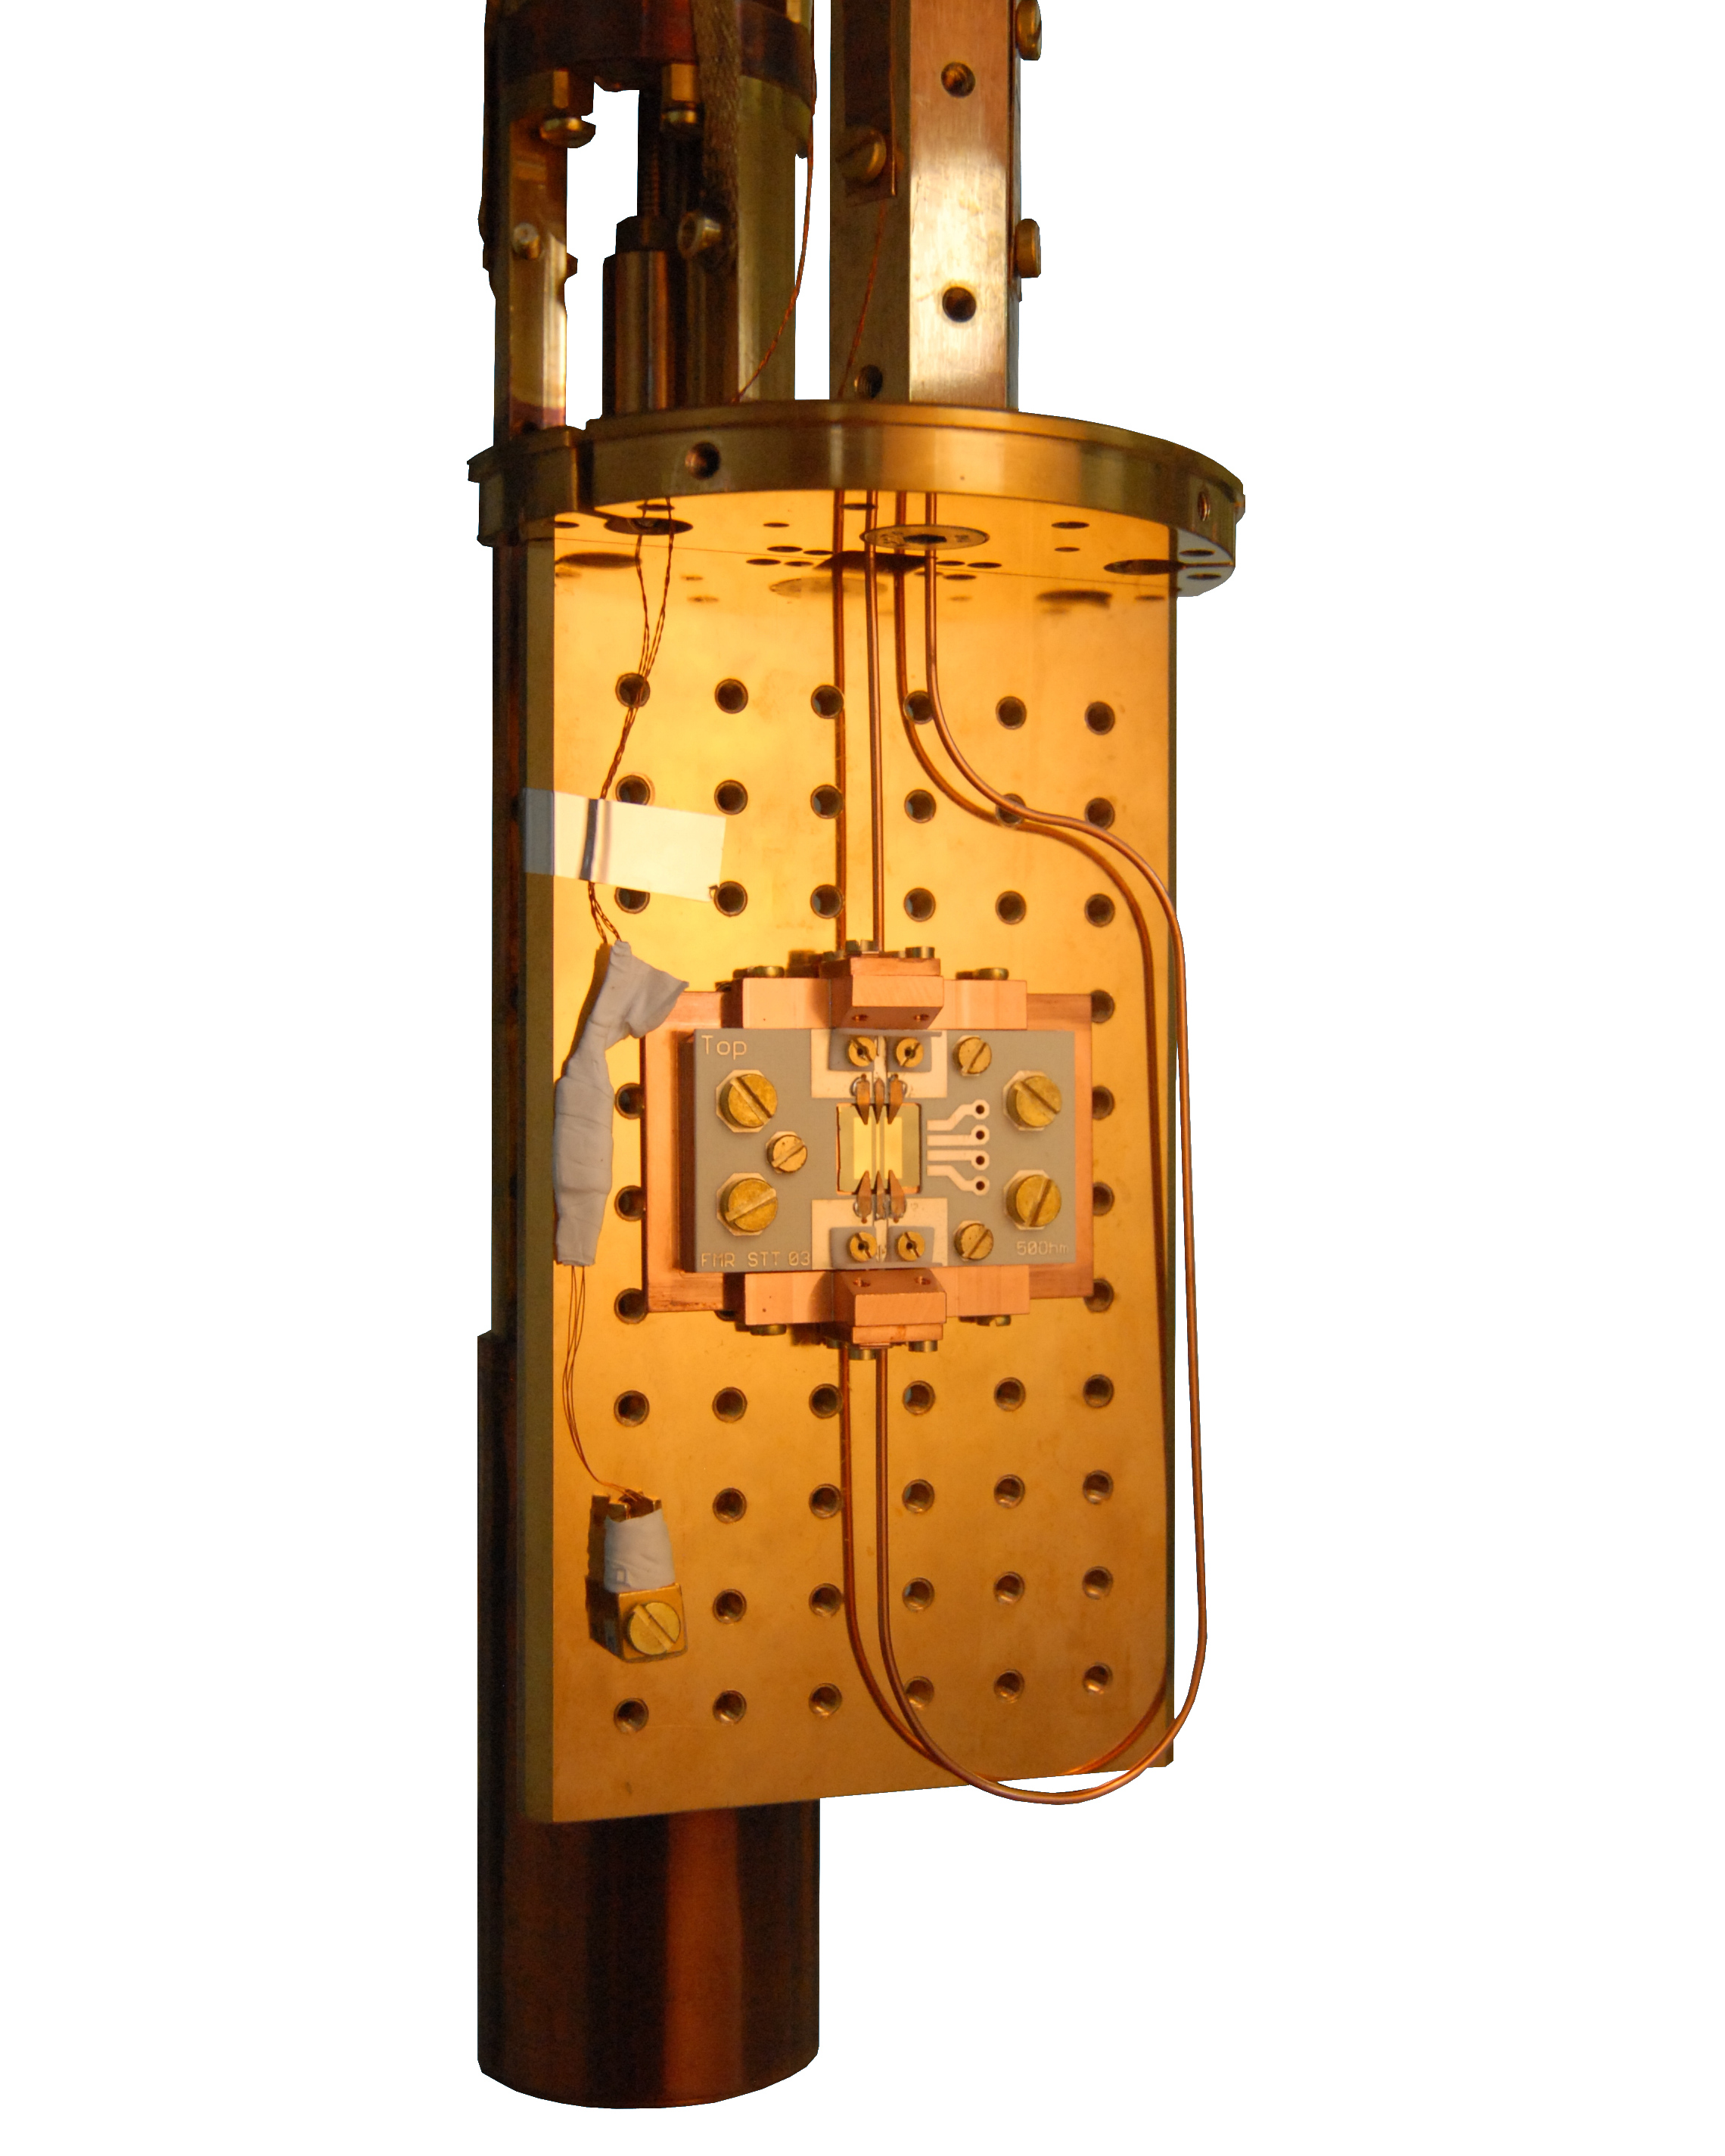
\includegraphics[width=\textwidth]{setup/holder/BF_freecut_45.jpg}
         \caption{BlueFors setup sample holder}
         \label{fig:setup_photo_bluefors}
     \end{subfigure}
     \begin{subfigure}[b]{.45\textwidth}
         \centering
         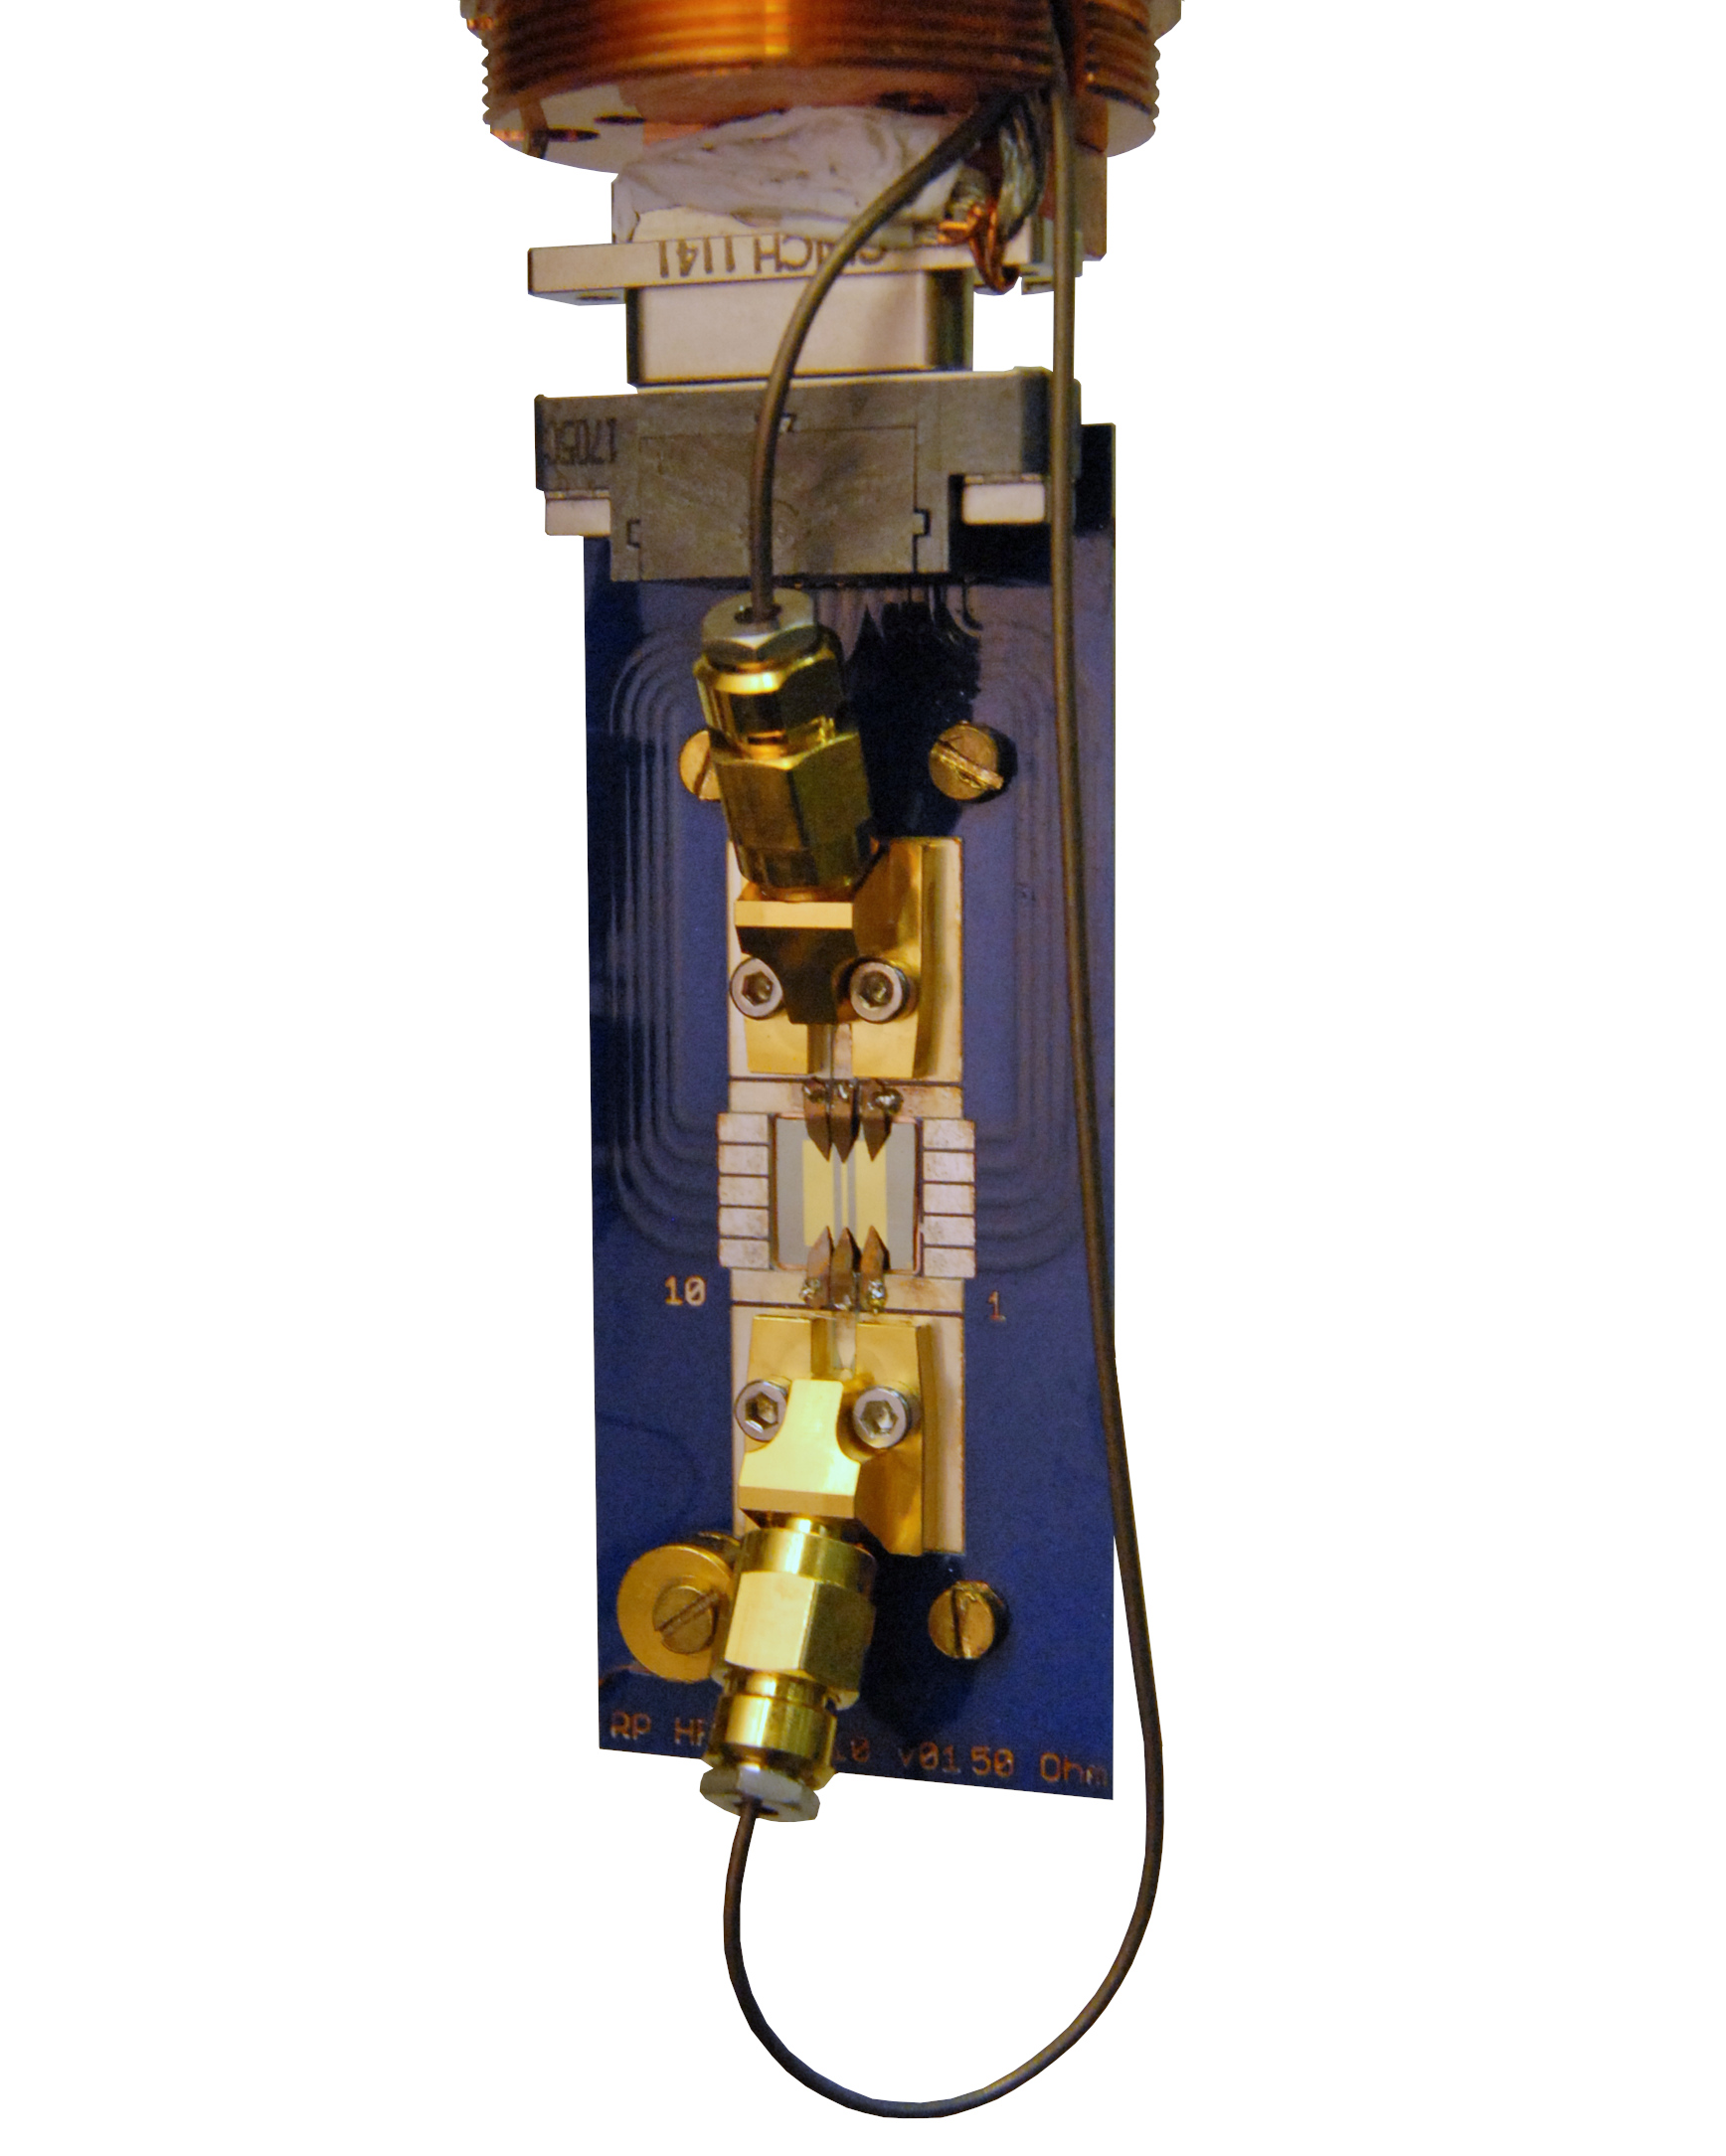
\includegraphics[width=\textwidth]{setup/holder/FH_freecut.jpg}
         \caption{HelioxVL setup sample holder}
         \label{fig:setup_photo_heliox}
     \end{subfigure}
        \caption[Sample holder pictures]{Sample holder pictures. \textbf{(a)} shows the FMR sample holder, with the mechanically controlled break junction setup in the background. Sample CPW3 is mounted. On the left side of the plate, the thermometer for $T_\text{FMR}$ is installed. \textbf{(b)} shows the sample holder of the Heliox setup. Beside the wave guide clamps, there are also bonding pads for direct current measurements. Again in the lower left, you can see the thermometer $T_\text{FMR}$ without any cables connected.}
        \label{fig:setup_photo}
\end{figure}

The HelioxVL setup in a wet cryostats, consisting of a $^3$He sample-in-vacuum dipstick and a dewar with built-in superconducting magnet. A thermometer is attached to the sample holder. The high-frequency cabling and the sample holder shown in Figure \ref{fig:setup_photo}b were realized in advance by Andreas Bloch and Lukas Kammermeier. The high-frequency cabling consist of copper cables for all setup parts with operating temperatures down to $4\,$K. For all parts with lower operating temperatures superconducting high frequency cables consisting of Nb/Ti are used.

The vector network analyzer (VNA) and pre-amplifier are mounted on a mobile rack for easy switching between setups. In addition, the room temperature thermometer and a measurement PC are mounted.

The VNA, both magnets, the room temperature thermometer and the thermometer of the HelioxVL Setup are controlled by the self-written program 'FMR control'. It is written in python3 and is mainly based on the packages pyvisa, numpy and matplotlib. It consists out of self-written device drivers and one central control program. By those drivers, the user can communicate with and control the devices. Several security features are implemented in them as well. Some device drivers can be found in the Appendix.

The measurement itself is run as multi-threading program, since recording the temperature, VNA and magnet control have to be done simultaneous. In general, at least one thread is recording the temperature the whole time. The logged temperature is averaged and then updated in a text file with corresponding timestamp. Another thread is controlling the magnet and VNA iteratively. Each iteration conducts the following operations. First, the magnet ramps to the desired field. Then the VNA measures the scattering parameter for all desired frequencies. A text file with the magnetic field, a timestamp and all the scattering parameter values and frequencies are saved. Afterwards these operations are conducted for the next desired magnetic field.
\chapter{Technical Findings}
At the beginning of this Chapter I want to clarify which quantities are measured. Then I will explain how the used measurement method works and how the signal processing is performed. After that I present what I did to optimize the signal. Later I will show what effect the ambient temperature has on the measurement. Further, I want to present the application of frequency domain reflectometry to find defects in the cabling. Finally, I will discuss the sample temperature dependence of the transmission.

Now we want to understand the measuring quantities of the vector network analyzer (VNA). It has two ports $i,j \in \{1,2\}$. Therefore, one can measure four so-called scattering parameters $S_{ij}$, which are connecting the incident\footnote{Commonly the outgoing and incident waves are defined in respect to the device under test. So $a$ is the output of the VNA, whereas $b$ is the measured wave amplitude at the VNA.} wave amplitudes $a$ with the outgoing wave amplitudes $b$, by
\begin{align}
    \left(\begin{array}{c}
         b_1\\
         b_2
    \end{array}\right)
    =
    \left(\begin{array}{cc}
         S_{11}&S_{12}\\
         S_{21}&S_{22}
    \end{array}\right)
    \cdot
    \left(\begin{array}{c}
         a_1\\
         a_2
    \end{array}\right)\,.
\end{align}

In general, we are interested in the transmission. Therefore, we will concentrate further in the forward transmission scattering parameter, defined by
\begin{align}
    S_{21}=\frac{b_2}{a_1}=|S_{21}| e^{\ima\phi_{21}}\,.
\end{align}
Since we compare two wave amplitudes we can calculate the respective maximum amplitude $|S_{21}|$ and the phase difference $\phi_{21}$ as well.

When we want to do further calculus we always have to keep in mind that $S_{21}$ is complex. So the absolute value and phase are given by
\begin{align}
    |S_{21}|&=\sqrt{\operatorname{Re}(S_{21})^2+\operatorname{Im}(S_{21})^2}\\
    \phi_{21}&=\operatorname{atan2}\left(\operatorname{Re}(S_{21}),\operatorname{Im}(S_{21})\right)\,.
\end{align}
The $\operatorname{atan2}$ operator is an extension of the inverse angle function $\operatorname{atan}$. If two Cartesian coordinates are passed as arguments to the $\operatorname{atan2}$ operator, the polar angle which is located in the correct quadrant is obtained. In consequence, the phase is given in a range of values from $0$ to $2\pi$.

When it comes to visualizing the scattering parameter, we will usually choose to plot the forward transmission $T_{21}$ in decibel (dB). It is calculated by
\begin{align}
    T_{21}=10\cdot \log_{10} \left( |S_{21}|^2 \right)
          =20\cdot \log_{10} \left( |S_{21}|\right)\,.
\end{align}

In the following, I am interested in the transmission depending on the angular frequency $\omega$ and magnetic field $H$. Since it is more convenient in technical applications to use the frequency $f$ with dimension Hertz (Hz), henceforth I will use $\omega/2\pi$, with dimension Hz\,\footnote{Since the typical frequencies are in the gigahertz regime, I will use GHz as unit.}. Likewise it is more convenient in technical applications, to express the magnetic flux density of a magnet in Tesla (T). Therefore, I will express the magnetic field $H$ in terms of $\mu_0H$, with unit T. \cite{ZNB40manual}

%%%%%%%%%%%%%%%%%%%%%%%%%%%%%%%%%%%%%%%%%%%%%%%%%%%%%%%%%%%%%%%%%%%%%%%%%%%%%%%%%%%%%%%%%%%%%%%
%%% Data processing
%%%%%%%%%%%%%%%%%%%%%%%%%%%%%%%%%%%%%%%%%%%%%%%%%%%%%%%%%%%%%%%%%%%%%%%%%%%%%%%%%%%%%%%%%%%%%%%
\section{Data Processing} \label{sec:data_processing}
%{\color{antiseeblau100}}
Now we want to understand how the measured scattering parameter is related to the susceptibility and how we can make the ferromagnetic resonance (FMR) observable.

First, we consider the raw measured scattering parameter $S_{21}$ as voltage ratio
\begin{align}
    S_{21}=\frac{V_\text{sys}+V_\text{ind}}{V_0}\,.
\end{align}
The voltage in the denominator $V_0$ is applied by the VNA, whereas the voltage in the numerator is a superposition of a systematic voltage $V_\text{sys}$ and of a CPW induced voltage $V_\text{ind}$.
The induced voltage is given by
\begin{align}
    V_\text{ind}=\ima\omega A\cdot V_0 \cdot \chi(\omega,H)\,,
\end{align}
where $A$ is a real-valued scaling parameter, that is dependent on the geometric dimensions of the co-planar waveguide (CPW) and the impedance of the entire system.

The systematic voltage is caused by the dielectric properties of the setup and depends only on the frequency. However, this voltage is much larger than the induced voltage. Since the FMR only affects the induced voltage, we have to consider it in the absence of the systematic voltage. That can be achieved by normalizing the measurement data by the normalization scattering parameter
\begin{align}
    S_{21}^0=\frac{V_\text{sys}}{V_0}\,.
\end{align}
With that in mind, we can write the normalized scattering parameter as
\begin{align}
    S_{21}^\text{n}=\frac{S_{21}}{S_{21}^0}=1+\frac{V_\text{ind}}{V_\text{sys}}\approx 1+\frac{V_\text{ind}}{V_0}\,.
\end{align}
Considering the induced voltage is way smaller than the voltage applied by the VNA $V_\text{ind}\ll V_0$ we can approximate $V_\text{ind}/V_\text{sys}\approx V_\text{ind}/V_0$.

Finally, our normalized scattering parameter is related to the susceptibility by
\begin{align}
    S_{21}^n=1+\ima\omega A\cdot \chi(\omega,H)\,.
\end{align}
Thus, the normalized scattering parameter no longer depends on the systematic voltage $V_\text{sys}$ or the voltage $V_0$ applied by the VNA. \cite{Louis2016}

Now that we understand how we relate the normalized scattering parameter to the susceptibility, we can address the signature of the FMR signal. From Chapter \ref{sec:theo_Kittel} we already know that the FMR frequency for an in-plane magnetized film is finite even in the absence of an external magnetic field. For applied fields the FMR frequency increases continuously. If negative fields are included, an axial symmetry to the zero-field line results. This leads to a typical curved \rotatebox[origin=c]{270}{$\pmb{\succ}$}-shape around the zero-field line, which becomes straighter for higher fields. The transmission decreases in the presence of the FMR.

The simplest method to determine the normalization scattering parameter is to find a frequency curve at a fixed magnetic field, which does not carry a FMR signal with certainty. Therefore, the maximum measured magnetic field $H_\text{n}$, where the FMR frequency is out of the measurement range is usually used for normalization. The normalization scattering parameter $S_{21}^0$ is then given by
\begin{align}
    S_{21}^0(\omega)=S_{21}(\omega, H_\text{n})\,.
\end{align}

The normalized scattering parameter $S_{21}^\text{n}$ and the normalized transmission $T_{21}^\text{n}$ are calculated by\footnote{Always keep in mind, that algebraic operations looks different for $T_{21}$ than for $S_{21}$, since they are logarithmic quantities.}
\begin{align}
    {S}_{21}^\text{n}&=\left.{S_{21}(\omega,H)}\,\middle/\, {S_{21}^0(\omega)}\right.\,,\label{eq:normS21}\\
    {T}_{21}^\text{n}&=T_{21}(\omega,H)-T_{21}^0(\omega)\,.
\end{align}

\begin{figure}
    \centering
    \import{analysis/really_small}{really_small.pgf}
    \caption[Raw and normalized transmission of sample CPW2]{Transmission $T_{21}$ of sample CPW2 depending on the frequency $\omega/2\pi$ and magnetic field $\mu_0H$. In \textbf{\color{antiseeblau100}a}, you can see the transmission $T_{21}^0$ for a fixed field at $H_\text{n}=1.1\,$T. In \textbf{\color{antiseeblau100}b} you can see a colorless grey scale map of the raw transmission $T_{21}$. In \textbf{\color{antiseeblau100}c} you can see a false color map of the normalized transmission $T_{21}^\text{n}$.}
    \label{fig:analysis_really_small}
\end{figure}
Figure \ref{fig:analysis_really_small} shows data obtained of sample CPW2 as an example for the normalization of the transmission. In panel a you can find the normalization transmission $T_{21}^0$, in panel b the raw transmission $T_{21}$ and in panel c the normalized transmission $T_{21}^\text{n}$. The \rotatebox[origin=c]{270}{$\pmb{\succ}$}-shaped FMR signal is clearly observable and not present at maximum field. At this point, I would like to emphasize the large amplitude ratio between raw and normalized transmission. The data range of the raw transmission covers approximately $60\,$dB, whereas the normalized transmission covers a data range of approximately $0.06\,$dB.

Now we want to turn to the quantitative evaluation of the FMR. In the following, I present an algorithm that provides reliable minima in the normalized transmission despite strong noise. The algorithm was applied to measurements of samples CPW2 and CPW3 and is visualized in Figure \ref{fig:analysis_kittel}.
\begin{figure}
     \centering
     \begin{subfigure}{\textwidth}
         \centering
         \import{analysis/kittel}{kittel_CPW2.pgf}\\
         \small\textbf{(1)} Sample: CPW2\\
         % [-1.48155226e+00  1.59066864e+04] [  3.82761252 426.54197394]
     \vspace{5mm}
     \end{subfigure}
     \begin{subfigure}{\textwidth}
         \centering
    \import{analysis/kittel}{kittel_CPW3.pgf}\\
         \small\textbf{(2)} Sample: CPW3\\
     \vspace{5mm}
         % [  32.43672464 9419.27273523] [ 12.12654013 586.13978913]
     \end{subfigure}
    \caption[Normalized transmission and minima of CPW2 and CPW3]{Normalized transmission and minima as a function of frequency $\omega/2\pi$ and magnetic field $\mu_0H$. The measurement of sample CPW2 is shown in \textbf{(1)} and of sample CPW3 is shown in \textbf{(2)}. Normalized transmission (false color) and minima found (\textbf{\color{antiseeblau100}magenta}) are shown in \textbf{\color{antiseeblau100}d}. Masked data areas are decolorized. In \textbf{\color{antiseeblau100}b}, the normalization transmission $T_{21}^0$ in \textbf{\color{seeblau100}blue} for $H_\text{n}=1\,$T can be seen. In \textbf{\color{antiseeblau100}a} and \textbf{\color{antiseeblau100}c}, the determined median curves $\langle\widetilde{T}_{21}^\text{n}(\omega)\rangle_H$ and $\langle\widetilde{T}_{21}^\text{n}(H)\rangle_\omega$ are plotted in \textbf{\color{seeblau65}light blue}.}
    \label{fig:analysis_kittel}
\end{figure}
First, I uniformly resized the datasets to a window from $0$ to $1\,$T and reduced the magnetic field resolution from $0.5\,$mT steps to $5\,$mT steps by averaging. Dataset CPW3 was cut off below $5\,$GHz, because there is no signal. Additionally, for this dataset, the frequency resolution was reduced from $20\,$MHz to $250\,$MHz by averaging. Now both datasets have the same resolution in frequency and magnetic field direction. Also the considered magnetic field section and the maximum frequency is the same. By averaging, some noise could already be reduced.

The normalized transmission $T_{21}^\text{n}$ is calculated as before using the normalization transmission $T_{21}^0$ at $H_\text{n}=1\,$T. Then I additionally normalize the transmission line-by-line to a range from $0$ to $1$ in arbitrary units\footnote{Since I am not working with quantitatively comparable transmissions, I use again $\widetilde{T}_{21}^\text{n}$ as notation}. Further, I form the median row-by-row $\langle\widetilde{T}_{21}^\text{n}(\omega)\rangle_H$ and subtract it from each row. These additional normalizations allow an effective reduction of frequency dependent noise. In magnetic field direction already subtracting the column-wise formed median $\langle\widetilde{T}_{21}^\text{n}(H)\rangle_\omega$ achieves a sufficiently good reduction of magnetic field noise. Then I mask frequency bands that are still highly noisy. Additionally, I mask data that are far away from the visible FMR signal.

Now minima are determined row-by-row and column-by-column. Its advantage is that many minima are obtained. The disadvantage is that some minima are lined up vertically or horizontally. Nevertheless, to prevent excessive weighting for horizontal or vertical features, I join the minima row-by-row and column-by-column. This means, e.g. that several minima obtained row-by-row at the same magnetic field are reduced to one minimum by averaging. The magnetization properties, which can be determined from the obtained minima, are discussed in Chapter \ref{chapter:physical_findings}.

%%%%%%%%%%%%%%%%%%%%%%%%%%%%%%%%%%%%%%%%%%%%%%%%%%%%%%%%%%%%%%%%%%%%%%%%%%%%%%%%%%%%%%%%%%%%%%%
%%% Modelling
%%%%%%%%%%%%%%%%%%%%%%%%%%%%%%%%%%%%%%%%%%%%%%%%%%%%%%%%%%%%%%%%%%%%%%%%%%%%%%%%%%%%%%%%%%%%%%%
\section{Modeling}
In this Section I will take the opportunity to present several other background treating methods, even though they did not yield better results than the already described method.

In another approach, instead of a fixed-field reference, as used in Section \ref{sec:data_processing}, a {moving-field reference} is used. We consider a small frame around the theoretically predicted resonance frequency $\omega_\text{res}^\text{theo}(H)$, with width $\Delta\omega_\text{f}$. So, we evaluate the scattering parameter solely in this field, given by
\begin{align}
    S_{21}^\text{f}=S_{21}(\omega_\text{res}^\text{theo}(H)\pm\Delta\omega_\text{f},H)\,.
\end{align}

As in Section \ref{sec:data_processing} discussed, I took the highest field within the given frame to obtain a reference curve. The normalization scattering parameter is given by
\begin{align}
    S_{21}^{\text{f},0}=S_{21}(\omega,H_\text{n})\,.
\end{align}

The normalized scattering parameter is calculated as before by
\begin{align}
    S_{21}^{\text{f},\text{n}}=S_{21}^\text{f}/S_{21}^{\text{f},0}\,.
\end{align}
You can see an example for the moving-field reference in Figure \ref{fig:analysis_mod}.3, right next to a fixed-field reference background treatment in Figure \ref{fig:analysis_mod}.1. \cite{maierflaig2017,siegl2020}
\begin{figure}
     \centering
     \begin{turn}{90}
     \begin{subfigure}[b]{3.65in}
         \hspace{.2in}
         \import{analysis/modelling}{dd.pgf}\\
         \centering\small\textbf{(2)} Derivative divide $\operatorname{d}_\text{D}S_{21}$\\
         %\caption{Derivative divide $\operatorname{d}_\text{D}S_{21}$}
         %\label{fig:analysis_mod_dd}
     \end{subfigure}
     \end{turn}
     \hspace{.2in}
     \begin{turn}{90}
     \begin{subfigure}[b]{3.65in}
         \hspace{.2in}
         \import{analysis/modelling}{U.pgf}\\
         \centering\small\textbf{(4)} Microwave permeability parameter $U(\omega)$\\
         %\caption{Microwave permeability parameter $U(\omega)$}
         %\label{fig:analysis_mod_U}
     \end{subfigure}
     \end{turn}
     \begin{turn}{90}
     \begin{subfigure}[b]{4in}
         \centering
         \import{analysis/modelling}{raw.pgf}\\
         \centering\small\textbf{(1)} Fixed-field reference method\\
         %\caption{Fixed-field reference method}
         %\label{fig:analysis_mod_raw}
     \end{subfigure}
     \end{turn}
     \hspace{.2in}
     \begin{turn}{90}
     \begin{subfigure}[b]{4in}
         \centering
         \import{analysis/modelling}{mrfm.pgf}\\
         \centering\small\textbf{(3)} Moving-field reference method\\
         %\caption{Moving-field reference method}
         %\label{fig:analysis_mod_mrfm}
     \end{subfigure}
     \end{turn}
    % \rotatebox[origin=c]{180}{$\omega/2\pi$ [GHz]}
    % $\mu_0H$ [T]
    % \rotatebox[origin=c]{180}{$\operatorname{Re}\left(\operatorname{d}_\text{D}S_{21}\right)\cdot 20$}
    % \rotatebox[origin=c]{180}{$\operatorname{Im}\left(U(\omega)\right)\cdot 10^4$}
    % \rotatebox[origin=c]{180}{$T_{21}^\text{n}$ [$0.01\,$dB]}
    % \rotatebox[origin=c]{180}{$T_{21}^\text{f,n}$ [$0.01\,$dB]}
    % \rotatebox[origin=c]{180}{$T_{21}^\text{f,0}$ [dB]}
    % $H_\text{n}=1.00\,$T
    % $H_\text{n}(\omega_\text{res}^\text{theo})$
    \caption[Comparison between different noise reduction methods for transmission data of sample CPW2]{Comparison between different signal enhancement methods for transmission data of sample CPW2, depending on the frequency $\omega/2\pi$ and the magnetic field $\mu_0H$. In \textbf{(1)} and \textbf{(3)} the two normalization methods fixed-field reference and moving-field reference are shown. In \textbf{\color{antiseeblau100}a} the normalization transmission is shown and in \textbf{\color{antiseeblau100}b} the normalized transmission. Additionally, the course of the magnetic field ${H}_\text{n}$ selected for normalization is shown in \textbf{\color{antiseeblau100}magenta}. \textbf{(2)} shows the real part of the derived scattering parameter $\operatorname{Re}\left(\operatorname{d}_\text{D}S_{21}\right)$. \textbf{(4)} shows the imaginary part of the microwave permeability parameter $\operatorname{Im}\left(U(\omega)\right)$.}
    \label{fig:analysis_mod}
\end{figure}

In comparison to the fixed-field method, the moving-field reference method has a slight advantage when it comes to line-by-line averaging. The drifts within one line are not that pronounced in comparison to the fixed-field normalization. You can see an example for line-by-line averaging in Figure \ref{fig:analysis_mod_avg}, in the Appendix. Due to the complexity of calculating the moving-field this method is not used further.

Next, I want to present the so-called 'derivative divide' method by Hannes Maier-Flaig \cite{maierflaig2018, maierflaig2017}. This method is particularly suitable for out-of-plane measurements, because then the FMR signal is strictly linear as function of the magnetic field. Even if this is true for high magnetic fields and in the in-plane case, this is not the case for smaller magnetic fields. Therefore, the application is not quite suitable, even though the method removes interfering temperature drifts and frequency dependencies without prior system calibration. The basic idea is to calculate the numerical deviation of the scattering parameter by
\begin{align}
    \operatorname{d}_\text{D}S_{21}=\frac{S_{21}(\omega,H+\Delta H_\pm)-S_{21}(\omega,H-\Delta H_\pm)}{S_{21}(\omega,H)\cdot\Delta H_\pm}\,,
\end{align}
where $\Delta H_\pm$ is the step width. We can easily show that $\operatorname{d}_\text{D}S_{21}=\operatorname{d}_\text{D}S_{21}^\text{n}$ holds true. Therefore, it makes no difference whether the raw or normalized scattering parameter is used to calculate the numerical derivative.

However, the deviated scattering parameter is related to the susceptibility by 
\begin{align}
    \operatorname{d}_\text{D}S_{21}&=\ima\omega A'\  \frac{\chi(\omega+\Delta\omega_\pm)-\chi(\omega-\Delta\omega_\pm)}{2\Delta\omega_\pm}\,,
\end{align}
where $\Delta\omega_\pm$ is the frequency step, given by approximately $\Delta\omega_\pm\approx\gamma\mu_0\Delta H_\pm$. You can find an application example in Figure \ref{fig:analysis_mod}.2. In advance the resolution of the data was strongly reduced by averaging in order to achieve the best visible results.

Finally, there is also the uncalibrated effective {microwave permeability} parameter
\begin{align}
    U(\omega)=\pm \ima \, \frac{\operatorname{ln}\left( S_{21}^n(\omega,H)\right)}{\operatorname{ln}\left( S_{21}^0(\omega,H)\right)}\,.
\end{align}
The sign is chosen in the way, that $\operatorname{Im}(U(\omega))$ is negative in the vicinity of the FMR peak. \cite{Kalarickal2006, Barry1986}

The susceptibility can be fitted by
\begin{align}
    U_\text{fit}(\omega)=C\left(1+\chi_0+\chi(\omega) e^{\ima\phi} \right)\,,
\end{align}
where $C$ is a real-valued scaling parameter, $\chi_0$ is a complex offset and $\phi$ is a phase shift. You can see an application example in Figure \ref{fig:analysis_mod}.4. \cite{maierflaig2018, maierflaig2017}

All these modeling approaches try to reduce background noise, depending on the frequency, but also apparently on the field. It is quite obvious that there is still significant noise left in the data. Therefore, I will discuss further signal optimization in the next Section and the obtained magnetization properties in Chapter \ref{chapter:physical_findings}. 

%%%%%%%%%%%%%%%%%%%%%%%%%%%%%%%%%%%%%%%%%%%%%%%%%%%%%%%%%%%%%%%%%%%%%%%%%%%%%%%%%%%%%%%%%%%%%%%
%%% Signal Optimization
%%%%%%%%%%%%%%%%%%%%%%%%%%%%%%%%%%%%%%%%%%%%%%%%%%%%%%%%%%%%%%%%%%%%%%%%%%%%%%%%%%%%%%%%%%%%%%%
\section{Signal Optimization}
In this Section I would like to present chronologically various results of my work that have a strong technical aspect and deal with signal optimization. First, I will start with the HelioxVL setup and present my findings on the hysteresis of the setup. Then the results obtained by this setup and the BlueFors setup will be compared. Afterwards, datasets that were recorded either in the frequency direction or in the magnetic field direction will be compared. Finally, the parameters I used will be discussed and recommendations for future measurements will be given.

%%%%%%%%%%%%%%%%%%%%%%%%%%%%%%%%%%%%%%%%%%%%%%%%%%%%%%%%%%%%%%%%%%%%%%%%%%%%%%%%%%%%%%%%%%%%%%%
%%% HelioxVL Hysteresis
\subsection{HelioxVL Setup Magnetization} \label{sec:analysis_hysteresis}
To gain a better understanding of the signals obtained in the HelioxVL setup, I performed several initial measurements. To this end, I performed fast, low-resolution measurements on sample CPW1.
Another aspect of these studies addresses the role of the field sweep directions and their possible advantages.

The results with the FMR typical \rotatebox[origin=c]{270}{$\pmb{\succ}$}-shape can be examined in Figure \ref{fig:analysis_hysteresis}. 
\begin{figure}
    \centering
    \import{analysis/hysteresis}{hysteresis.pgf}
    % {\color{seeblau100}$\pmb{\leftarrow}$} $\mu_0H$ [T]
    \caption[Normalized transmission data in down and up sweep direction]{Normalized transmission $T_{21}^\text{n}$ in down ({\color{seeblau100}$\pmb{\leftarrow}$}, \textbf{\color{antiseeblau100}a}) and up ({\color{seeblau100}$\pmb{\rightarrow}$}, \textbf{\color{antiseeblau100}b}) sweep direction in dependence of frequency $\omega/2\pi$ and magnetic field $\mu_0H$ of CPW1 measured at the HelioxVL setup, initially magnetized at $3\,$T. In addition, dashed lines in \textbf{\color{antiseeblau100}magenta} have been added for visual emphasis.}
    \label{fig:analysis_hysteresis}
\end{figure}
After a $+3\,$T initialization I started the measurement first at $+320\,$mT (down sweep, {\color{seeblau100}$\pmb{\leftarrow}$}, panel a) and then at $-320\,$mT (up sweep, {\color{seeblau100}$\pmb{\rightarrow}$}, panel b).

It is easy to see that the center of the \rotatebox[origin=c]{270}{$\pmb{\succ}$}-shaped FMR signal is shifted by $+4\,$mT towards zero in the down sweep, whereas in the up sweep the \rotatebox[origin=c]{270}{$\pmb{\succ}$}-shape is exactly occurring at $0\,$mT. It is conceivable that the magnet has a small offset, but as well that components of the cryostat can be magnetized. A frequency independent feature can be observed in both measurements. In the case of the up sweep, it is at $+8\,$mT and in the the down sweep at $-1\,$mT. What is the cause of this feature has not been investigated further. However, this also speaks for a hysteretic magnetization effect. We were able to determine that the SK connector of the measurement line are ferromagnetic and are very likely responsible for this hysteric magnetization.
%Since the volume of the examined Co is simply too small to induce such magnetization effects, this effect must come from the setup itself. It is known that the magnets used can also have a small offset. However, we were able to determine that the SK connector of the measurement line are ferromagnetic and are very likely responsible for this hysteric magnetization.

For future measurements initialization has been omitted, as I have also measured with way stronger magnetic fields. I assume that magnetic fields around $1\,$T are sufficient to neglect any magnet training effects. So, inherent down sweeps from the initially applied magnetic field are measured. Of course this can still be varied in sign.

%%%%%%%%%%%%%%%%%%%%%%%%%%%%%%%%%%%%%%%%%%%%%%%%%%%%%%%%%%%%%%%%%%%%%%%%%%%%%%%%%%%%%%%%%%%%%%%
%%% Setup comparison
\subsection{Comparison of the Setups Used}
Finally, one focus of my work was to reproduce the FMR measurements in the HelioxVL setup. This measurements were already done previously in the BlueFors setup by Sergej Andreev. To this end, I wanted to use a sample with the strongest potential signal. Since this depends on the volume, I used CPW1 already described in Section \ref{sec:sample_design}.

Even though both measurements use very different measurement parameters and different sweep types, they can be compared qualitatively. The measurement at the BlueFors was done with Sergej Andreev's measurement program. This measurement method is explained in detail in Section \ref{sec:hf_sweep}. 

Panel a of Figure \ref{fig:analysis_setup_comp} shows the normalization transmissions, obtained at a magnetic field $H_\text{n}=315\,$mT.
\begin{figure}
    \centering
    \import{analysis/setup_comp}{setup_comp.pgf}
    \caption[Normalized transmission of sample CPW1 at the setups HelioxVL and BlueFors]{Normalized transmission $\widetilde{T}_{21}^\text{n}$ of the same sample CPW1 in the setups HelioxVL (\textbf{\color{antiseeblau100}b}) and BlueFors (\textbf{\color{antiseeblau100}c}) in dependence of frequency $\omega/2\pi$ and magnetic field $\mu_0H$. In panel \textbf{\color{antiseeblau100}a} the normalization transmissions $\widetilde{T}_{21}^0$ in \textbf{\color{antiseeblau100}magenta} and \textbf{\color[rgb]{0.878733401483036, 0.49928686449731624, 0.7675654756534815}light magenta} at $H_\text{n}=315\,$mT are shown.}
    % H=.315
    \label{fig:analysis_setup_comp}
\end{figure}
In magenta, the raw transmission measured in the HelioxVL setup and in light magenta, the already zero-field calibrated transmission measured in the BlueFors setup is shown. The normalized transmission measured in the HelioxVL and BlueFors setup is shown in panel b and c. 

Even though both measurements are different in noise shape and noise intensity due to the different parameter and sweep types, the \rotatebox[origin=c]{270}{$\pmb{\succ}$}-shape typical for FMR is recognizable. Despite all this, it can be said with certainty that FMR measurements can be made on both setups.

%%%%%%%%%%%%%%%%%%%%%%%%%%%%%%%%%%%%%%%%%%%%%%%%%%%%%%%%%%%%%%%%%%%%%%%%%%%%%%%%%%%%%%%%%%%%%%%
%%% hf sweep
\subsection{Magnetic Field and Frequency Sweep method} \label{sec:hf_sweep}
Usually, the VNA measures the scattering parameters for all set frequencies in a single sweep\footnote{Even though this is called a sweep, the VNA measures per default in a so called stepped method. Here each frequency is set before measurement and is changed just after the measurement. \cite{ZNB40manual}}. Therefore, it seems only natural to set a fixed magnetic field and then measure a frequency sweep. In the following, I will refer to this procedure as frequency sweep method.

However, also with a fixed frequency, the magnetic field can be swept. Henceforth, I will call this method the magnetic field sweep method. This method was previously implemented by Sergej Andreev and measured with his measuring program.

The measurement procedure of the magnetic field sweep method differs from the frequency sweep method in that a zero-field calibration is carried out first. At this point, the magnet is given a sweep rate and target. As the magnetic field changes continuously, the VNA measures miniate frequency sweeps, with a small span around a center frequency.  The collected data, magnetic field, frequency, transmission and phase are then averaged to obtain a data point. For visualization, a binning algorithm is also used later, in which transmission and phase are averaged again.

A problem that should not be underestimated is the averaging. As I mentioned in the beginning, the transmission is a logarithmic quantity. Therefore the scattering parameter needs to be used to calculate a mean value instead and calculate the transmission from that, as
\begin{align}
    T_{21}\left(\overline{S_{21}}\right) &= 20\cdot \log_{10} \left( |\overline{S_{21}}|\right) \\
    &= 20\cdot \log_{10} \left( \left|\frac{1}{N}\sum_{i=0}^N{S_{21,i}}\right|\right)\,.
\end{align}

However, calculating the mean of the transmission directly, can be traced back to a geometric mean of the magnitude of the scattering parameter, like
\begin{align}
    \overline{T_{21}}&= \overline{20\cdot \log_{10} \left( \left|{S_{21}}\right|\right)}\\
    &= \frac{20}{N}\cdot \sum_{i=0}^N\log_{10} \left( \left|{S_{21}}\right|\right)_i\\
    &= 20 \cdot \log_{10} \left( \prod
    _{i=0}^N\sqrt[N]{\left|{S_{21}}\right|_i}\right)\,.
\end{align}

Fortunately, the transmission values within a miniate sweep and between neighbouring data points do not differ much. Considering this, the geometric mean and arithmetic mean are quite close to each other. Therefore, it is still possible to discuss semi-quantitatively. Larger differences can only be found, if there are strong outliers among the values, which is why the geometric mean is often used as a noise filter. I will use $\widetilde{T}_{21}$ when the geometrically and arithmetically averaged transmission values are compared. \cite{gonzalez2008}

Superconducting magnets, as we use them, can only be swept very slowly. This results in a disadvantage of the magnetic field sweep method with respect to the measurement speed. Thus, at a constant frequency the field is swept up at maximum rate and then swept down again. During this process it is possible to measure well. However, there is no great information gain to measure up and down sweep each time.

In Figure \ref{fig:analysis_hf_sweep} a comparison of two measured down sweeps is made between frequency sweep method (panel b) and with magnetic field sweep method (panel c). 
\begin{figure}
    \centering
    \import{analysis/hf_sweep}{hf_sweep.pgf}
    \caption[Normalized transmission of sample CPW2 in frequency and magnetic field sweep method]{Normalized transmission $\widetilde{T}_{21}^\text{n}$ of the same sample CPW2 at the BlueFors setup in frequency sweep method (\textbf{\color{antiseeblau100}a}) and magnetic field sweep method (\textbf{\color{antiseeblau100}b}) in dependence of frequency $\omega/2\pi$ and magnetic field $\mu_0H$. Panel \textbf{\color{antiseeblau100}a} shows the normalization transmissions $\widetilde{T}_{21}^0$ in \textbf{\color{antiseeblau100}magenta} and \textbf{\color[rgb]{0.878733401483036, 0.49928686449731624, 0.7675654756534815}light magenta} at $H_\text{n}=1.05\,$T.}
    % H=1.05
    \label{fig:analysis_hf_sweep}
\end{figure}
The up sweep dataset of the magnetic field sweep method is available, but does not provide any additional relevant information and is therefore not shown. 

So, for each frequency a whole up and down sweep of the magnetic field has to be repeated. With limited measurement time the frequency resolution is therefore severely limited. Thus, in Figure \ref{fig:analysis_hf_sweep}c a frequency step size of $250\,$MHz can be seen, with a total measurement time of about $200\,$h.

With the frequency sweep method, on the other hand, there are more options regarding the parameters. A higher frequency resolution of $20\,$MHz is usually used. However, the two measurements seen in Figure \ref{fig:analysis_hf_sweep} were made with the same parameters such as resolution and range. By repeatedly averaging the same frequency sweep at the same field, the frequency sweep method could be slowed down to a total measurement time of about $75\,$h for a down sweep dataset. With well comparable FMR signals between magnetic field sweep method and frequency sweep method the frequency sweep method is clearly faster.

Finally, I want to talk about another not that obvious advantage of the frequency sweep method. When it comes to noise apparently the frequency sweep measurement in Figure \ref{fig:analysis_hf_sweep}b has additional noise. In both measurements horizontal lines can be seen, most likely due to frequency depending effects. However, in the frequency sweep method additionally vertical lines appear. Since we can exclude magnetic dependencies by the magnetic field sweep measurement, we have to assume, that some time dependent noise is disturbing the measurement. This time-dependent noise is included in both measurements but can only be resolved separately from frequency-dependent noise in the frequency sweep method. In the next Section, this time-dependent noise will be explained in more detail.

%%%%%%%%%%%%%%%%%%%%%%%%%%%%%%%%%%%%%%%%%%%%%%%%%%%%%%%%%%%%%%%%%%%%%%%%%%%%%%%%%%%%%%%%%%%%%%%
%%% Temperature induced noise
\subsection{Noise Induced by the Laboratory Temperature} \label{sec:analysis_temp}
In this Section I would like to talk about temperature induced noise. I could show that the room temperature in laboratory P10 varies up to $2\,^\circ$C. This significantly disturbs the BlueFors measurement electronics, consisting of VNA and pre-amplifier.

Essentially, I made three measurements to show the laboratory temperature induced noise. The results of these measurements are shown in Figure \ref{fig:analysis_temp}. 
\begin{figure}
    \centering
    \import{analysis/temp}{temp.pgf}
    % $T_\text{RT}$ [$^\circ$C]
    % $\widetilde{T}_{21}^\text{n}$ [$0.01\,$dB]
    \caption[Normalized transmission over frequency and as well as temperature over time]{Normalized transmission $T_{21}^\text{n}$ over frequency $\omega/2\pi$ and as well as temperature over time $t$. The temperature is either measured in the laboratory $T_\text{RT}$ or the box $T_\text{box}$, used for isolation. For normalization the last transmission $T_{21}^0(t_\text{max})$ was used. \textbf{\color{antiseeblau100}a}, \textbf{\color{antiseeblau100}b} \& \textbf{\color{antiseeblau100}c} are showing the measurements without, with and with tempered pre-amplifier.}
    \label{fig:analysis_temp}
\end{figure}

For measurement one I connected the output and input of the VNA and measured the transmission for all set frequencies, shown in Figure \ref{fig:analysis_temp}a. For measurement two I connected the pre-amplifier in between, shown in Figure \ref{fig:analysis_temp}b. Measurement three is shown in Figure \ref{fig:analysis_temp}c and is made with a temperature stabilization\footnote{The stabilization consists out of a temperature controller and a styrofoam box for isolation. The temperature controller was built by Sergej Andreev and consists out of a Peltier element and a water cooling system. This setup can control the pre-amplifier to stable $25\,^\circ$C.}, to control the temperature of the pre-amplifier. Simultaneously, I logged either the room temperature $T_\text{RT}$, or the temperature within the styrofoam box $T_\text{box}$, used for isolation. 

Besides a regular fluctuation of the room temperature in measurements one and two in a $0.5$ to $1\,$h cycle, a particularly strong fluctuation occurs every $10$ to $12\,$h. I guess this has to do with the air conditioning of the laboratory. Furthermore, a low frequent fluctuation with a period of $24\,$h can be observed. This means that the laboratory temperature depends slightly on the time of day. The high frequency fluctuations in measurement two are way more irregular in amplitude. This can be explained by the fact that the temperature is more stable at weekends (measurement one) compared to during the week (measurement two) with higher numbers of people in the laboratory.

Measurement one without a pre-amplifier shows that the transmission varies together with the temperature. To compare the fluctuation quantitatively I calculated the average value column-by-column and then calculated the standard deviation $\sigma$ (STD) of both the transmission and the temperature. The room temperature has a STD of $\sigma(T)=0.53\,^\circ$C. The transmission has a STD of $\sigma(\langle T_{21}\rangle_\omega)=3.9\cdot10^{-3}\,$dB. Calculating the ratio of these we get $\sigma(\langle T_{21}\rangle_\omega)/\sigma(T)=7.3\cdot10^{-3}\,$dB/$^\circ$C, which is even slightly better than the specified drift of $0.01\,$dB/$^\circ$C for the VNA. \cite{ZNB40brochure}

In measurements two and three, frequency bands with different temperature-dependent transmission characteristics appear. Especially in the higher-frequency third, temperature-dependent transmission fluctuations are clearly visible. Especially the day-dependent temperature fluctuations seem to have a strong effect on the transmission. The transmission in measurement two is significantly higher in the first $\approx15\,$h. This can be explained by a self-induced heating-up of the pre-amplifier to a stable operating temperature.

Quantitatively, the STD of transmission in the whole measurement two is $\sigma(\langle T_{21}\rangle_\omega)=4.7\cdot10^{-2}\,$dB, in the second half of measurement two the STD is $\sigma(\langle T_{21}\rangle_\omega)=1.3\cdot10^{-2}\,$dB and in measurement three the STD is $\sigma(\langle T_{21}\rangle_\omega)=1.6\cdot10^{-2}\,$dB. It would be interesting to know how much the laboratory temperature varied during measurements three, since the transmission varies more than in the second half of measurement two. However, it can be deduced from the box temperature $T_\text{box}$ that the cooling of the pre-amplifier works reliable. The temperature fluctuations are characterized by the course of the day, which suggests a cooling water temperature fluctuation.

Only from the transmission noise perspective the further use of the pre-amplifier is not recommended. Nevertheless, its usage is recommended especially at higher frequencies, since the signal gain of the pre-amplifier outweighs the higher noise. For comparison two measurements with and without tempered pre-amplifier are shown in Figure \ref{fig:analysis_temp_lowbw}, in the Appendix.

%%%%%%%%%%%%%%%%%%%%%%%%%%%%%%%%%%%%%%%%%%%%%%%%%%%%%%%%%%%%%%%%%%%%%%%%%%%%%%%%%%%%%%%%%%%%%%%
%%% How to parameter
\newpage
\subsection{Parameter Study} \label{sec:parameter_study}
In this Section I would like to make recommendations for the parameter space to be chosen. Often enough, the measurement time is limited and cannot be increased arbitrarily. Here I mainly refer to the magnets, the VNA and the pre-amplifier used.

Magnetic fields can be adjusted in steps of down to $0.5\,$mT and I would also recommend working with that stepsize. For fast measurements you can also increase to $1\,$mT steps. From Section \ref{sec:analysis_hysteresis} we know that asymmetries can arise around $0\,$T, so  measurements should also be made generously around $0\,$T. The maximum frequency used of the VNA is $40\,$GHz, with the gyromagnetic ratio of about $28\,$GHz/T, the upper FMR limit for nearly spherical geometries is about $1.4\,$T. In practice, it has turned out that only fields up to $1.1\,$T are interesting, since in-plane measurements are conducted. Summarizing, I would recommend a measurement between -$50\,$mT and $1.2\,$T in $0.5\,$mT steps, which corresponds to $2501$ measuring points in magnetic field direction. \cite{AM430manual,IPS12010manual}

The VNA provides a frequency range from $100\,$kHz to $40\,$GHz, which in general I would always use. For faster measurements the frequency can be cut off below the upper limit. Thus, the signal strength for high frequencies also decreases strongly, e.g. in Section \ref{sec:analysis_temp}, I only measured up to $26\,$GHz. In combination with the pre-amplifier measurements should only be taken from $2\,$GHz, as this only supports frequencies between $2$ to $50\,$GHz. The number of measurement points is almost arbitrary\footnote{Technically it is limited to $100001$ points by the VNA. However, you can split your sweep into several sub-sweeps. Doing so the number of points can increase significantly.}. Therefore, the increase in total measurement time has to be considered. In practice around $2000$ points have proven to be useful.
I would suggest measurements between $2\,$GHz and $40\,$GHz, in $20\,$MHz steps. That corresponds to $1901$ measuring points in frequency direction. \cite{ZNB40manual,U7227manual}

With an image resolution of $2501\times1901$ points, it is easy to zoom into features afterwards. Also, a smoother image can be achieved by averaging afterwards.

Unfortunately, no reliable numbers on the relationship between bandwidth and dynamic range can be found in the VNA specifications. However, it is certain that the smaller the bandwidth, the better the resolution for small signal strengths. However, with a smaller bandwidth the measurement time increases. Averaging over several frequency sweeps helps as well against noise, which also increases the measurement time. While in the end it is always a question of weighing measuring time against signal strength, in practice, it has been shown that a bandwidth of $1\,$kHz and $10$ averages yields satisfying results, when the pre-amplifier is used. If you want to measure without a pre-amplifier, a bandwidth of about $30\,$Hz and $3$ averages is recommended. In general, the use of the pre-amplifier is recommended, especially for frequencies above $30\,$GHz. \cite{ZNB40manual,ZNB40brochure,ZNB40spec}

%%%%%%%%%%%%%%%%%%%%%%%%%%%%%%%%%%%%%%%%%%%%%%%%%%%%%%%%%%%%%%%%%%%%%%%%%%%%%%%%%%%%%%%%%%%%%%%
%%% FDR
\begin{figure}[t]
    \centering
    \import{analysis/FDR}{fdr2.pgf}
    \caption[Reflection parameters as a function of resonator length]{Reflection parameters $\hat{R}_{11}$ \& $\hat{R}_{22}$ in panel \textbf{\color{antiseeblau100}a} \& \textbf{\color{antiseeblau100}b} as a function of resonator length $d$. Three measurements each at \textbf{\color[rgb]{0.000000,0.404312,0.680182}$\mathbf{4}$\,K}, \textbf{\color[rgb]{0.085109,0.628859,0.828930}$\mathbf{161}$\,K} and \textbf{\color[rgb]{0.499287,0.767565,0.878733}$\mathbf{285}$\,K} are shown. The maximum of the dominant wide peaks are marked in \textbf{\color{antiseeblau100}magenta} at $57.4\,$cm and $54.9\,$cm.}
    \label{fig:analysis_tdr}
    % $T_\text{FMR}=4\,$K
    % \,$54.9\,$cm
\end{figure}

\section{Frequency Domain Reflectometry}

Frequency domain reflectometry (FDR) is a commercially available, powerful software for analyzing transmission lines with a VNA. I utilized the measured reflection scattering parameters to find wiggle contacts by applying a fast Fourier transform myself. Since this technique was implemented by Smith-Rose in the 1930s, more sophisticated reconstruction algorithms have been put forward. Because a limited understanding of this technique will suffice in the following, I will not go into detail. More information can be found following sources, \cite{smithrose1933, vanhamme1990, shin2005, keysightFDR}.

The reflection scattering parameter $S_{ii}, i\in\{1,2\}$ is defined by
\begin{align}
    S_{ii}=\frac{b_i}{a_i}\,.
\end{align}

The VNA measures the scattering parameter as a function of frequency. From frequency domain to the time domain can be switched by applying the symmetrized ortho-normalized fast Fourier transformation
\begin{align}
    \hat{S}_{ii}(t)=\operatorname{FFT}\left( S_{ii}(f)\right)\,.
\end{align}

Now I rescale the time-axis to get the typical resonator length $d$, by
\begin{align}
    \Delta d = \frac{c_0/\sqrt{\varepsilon_\text{r}}}{2\cdot 2\pi\Delta f}\,.
\end{align}
Here is $c_0$ the speed of light and the factor of propagation velocity can be approximated as $1/\sqrt{\varepsilon_\text{r}}\approx 0.70-0.77$ for common microwave cables, where $\varepsilon_\text{r}$ is the relative permittivity. A factor of 2 is inserted, on account of the typical resonator length and not the path length is to be considered. \cite{HS2020, elspec}

Finally, the reflection parameter in decibels is calculated by
\begin{align}
    \hat{R}_{ii}(d)=20\cdot \log_{10}\left(|\hat{S}_{ii}(d)|\right)\,.
\end{align}

In the following, I will use an example to explain the possibility of finding a loose contact in the transmission line. The transmission has drastically decreased in the course of a cooling process. I have carried out three reflection measurements during the warm-up process. 

The first measurement was made at $4\,$K, the second at $161\,$K. The high temperature superconducting cables used in some sections are superconducting only up to about $75\,$K, see next Section \ref{sec:analysis_fT_map}. The transmission during the first two measurements were significantly worse than I would usually expect and leads me to the conclusion that the transmission line is interrupted. The last measurement was taken near room temperature at $285\,$K. At this temperature I was able to measure the expected transmission and I can assume that the transmission line is intact again.

The respective reflection parameters $\hat{R}_{11}$\,\&\,$\hat{R}_{22}$ as a function of resonator length $d$ can be seen in Figure \ref{fig:analysis_tdr}. The reflection parameters at $4\,$K and $161\,$K did not differ significantly from each other in their magnitudes and are referred as interrupted state in the following. The reflection parameters at $285\,$K in intact state differs significantly from the other reflection parameters measured.

The first two strong peaks are formed at resonator lengths corresponding to the distance between the $-10\,$dB dampers of the setup and the adjacent connectors. The second peak, like most of the following peaks, looks like double peaks. This can be explained by the placeholders that are built in instead of the original dampers. The placeholders and the next cable termination form two resonators of only slightly different length. The following peaks corresponding to resonator length up to $50\,$cm can all be explained by resonances in the different cable parts.

Around a resonator length of $57.4\,$cm, respectively $54.9\,$cm a broad peak builds up in the interrupted state measurements. This resonator length corresponds to the cable Sections between the sample holder and the mixing chamber (MXC). There is a significant difference in magnitude between the interrupted and intact state of the cables. From this difference I conclude that the interruption of the transmission line must be at the cable connection to the PCB\footnote{The inner conductor pressed onto the PCB board was stripped too tightly and pulled off the PCB board when it cooled down. I was able to fix this by stripping the inner conductor again generously.}. However, even in the intact state, the peaks corresponding to the same resonator length, are still higher than most of the peaks corresponding to smaller lengths. This is again to be expected since the inner conductors of the cable are simply pressed onto a PCB board in the sample holder, thus a higher reflection is assumed than within a commercial connector.
I attribute the peaks at higher resonator lengths, to higher resonance orders. 

In summary, I could show that with the measurement of both reflection scattering parameters in interrupted and intact state, a localization of a interruption in the transmission line is possible just by using the VNA.

%%%%%%%%%%%%%%%%%%%%%%%%%%%%%%%%%%%%%%%%%%%%%%%%%%%%%%%%%%%%%%%%%%%%%%%%%%%%%%%%%%%%%%%%%%%%%%%
%%% T(T)
\section{Transmission Dependency on Sample Temperature} \label{sec:analysis_fT_map}
Since I measured at low temperatures, between $50\,$mK and $4\,$K, I am also interested in changes of the transmission over the temperature. For this reason, I constantly logged the transmission and temperature of sample CPW3 during a warm-up process. The results can be seen in Figure \ref{fig:analysis_fT_map}.
\begin{figure}
    \centering
    \import{analysis/fT_map}{fT_map.pgf}
    \caption[Transmission behavior of sample CPW3 over temperature during warm-up]{Transmission behavior of sample CPW3 over temperature $T_\text{DUT}$ during warm-up process. In panel \textbf{\color{antiseeblau100}a} you can see the normalization transmission at $7\,$K. In panel \textbf{\color{antiseeblau100}b} the normalized transmission $T_{21}^\text{n}$ over the complete temperature range is shown. Four insets for close-ups are included as well.}
    \label{fig:analysis_fT_map}
\end{figure}

Since the thermometer of the sample holder ($T_\text{FMR}$) is not calibrated up to room temperature, in comparison to the magnet thermometer ($T_\text{magnet}$), the device under test (DUT) temperature $T_\text{DUT}$ was calculated by
\begin{align}
    T_\text{DUT}(t)=\left(\frac{1}{2}+\operatorname{atan}\left(\frac{t-t_0}{\Delta t}\right)\right)\cdot T_\text{FMR}(t)+\left(\frac{1}{2}-\operatorname{atan}\left(\frac{t-t_0}{\Delta t}\right)\right)\cdot T_\text{magnet}(t)\,.
\end{align}
The parameters $t_0$ and $\Delta t$ were chosen so that when the two measured temperatures begin to diverge at about $25-30\,$K, $T_\text{DUT}$ begins to converge from $T_\text{FMR}$ to $T_\text{magnet}$. This was visualized for a typical warm-up curve in Figure \ref{fig:analysis_fT_map_Tt}.
\begin{figure}
    \centering
    \import{analysis/fT_map}{T(t).pgf}
    \caption[Typical warm-up curve for the BlueFors setup]{Typical warm up curve over time of the BlueFors setup. \textbf{\color{seeblau100}$\boldsymbol{T}_\text{FMR}$} \& \textbf{\color[rgb]{0.571821,0.803166,0.878400}$\boldsymbol{T}_\text{magnet}$} are measured temperatures, whereas \textbf{\color{antiseeblau100}$\boldsymbol{T}_\text{DUT}$} is calculated by those temperatures and some $\operatorname{atan}$ weights. Panels \textbf{\color{antiseeblau100}a} \& \textbf{\color{antiseeblau100}b} are showing different time periods. The parameters are $t_0\approx4\,$h and $\Delta t\approx20\,$min} 
    \label{fig:analysis_fT_map_Tt}
\end{figure}

The most dominant feature in Figure \ref{fig:analysis_fT_map} is the smooth transition at about $75\,$K from a very homogeneous transmission distribution, given by normalization, to a rougher transmission distribution. This behavior can be explained very well by the collapse of superconductivity in the used high temperature superconducting microwave cables.

The vertical features at around $180\,$K are attributed to binning-algorithm errors and will not be discussed further.


Next, I would like to discuss features that need further investigation. For some frequencies, better transmission is obtained at higher temperatures, when the superconducting cables are in normal state. These features seem to be associated with a temperature dependence of the frequency. In particular, the frequency and temperature dependent features are magnified in the four insets of Figure \ref{fig:analysis_fT_map}. In itself, the FMR has no temperature dependent quantities, so these features must also be related to the transmission characteristics of the microwave cables.

An approach to explanation would be to assume an electro-magnetic resonator. In this case, the permittivity of the resonator would have to depend strongly on the temperature. Since the structure is in vacuum, only the cables and their terminations can form resonators, which depend on temperature and frequency.

At this point, further investigation is needed to determine the origin of these features. Also, a higher resolution measurement in the range from base temperature to about $10\,$K would be very interesting. In this temperature range, I expect a large number of interesting transmission features, especially in the order of magnitude of transmission variations due to FMR. Here I would like to emphasize the different orders of magnitude of transmissions variation caused by either temperature variations or typically measured FMR. Unfortunately, the measured warm-up was too fast for the slow frequency sweeps, which are optimized for a high dynamic range of transmission. Further, parameter optimization is needed for measurements in this low temperature range.

In early measurements on the HelioxVL setup I could see large differences in transmission compared to the FMR signal before and after helium transfer. During the transfer, the temperature in the dewar fluctuates quite a lot. Unfortunately, I did not log the temperature during these measurements and it remains questionable whether the presence of the transfer line might not also influence the applied magnetic field.
\chapter{Results and Diskussion} \label{chapter:physical_findings}
In this Chapter, I will compare two datasets recorded for samples CPW2 and CPW3. Although many parameters differ in sample preparation and data collection (see Table \ref{tab:analysis_kittel} in the Appendix), these two samples are interesting for investigating the effect of two different Co thicknesses $d_\text{CPW2}=32.5\,$nm \& $d_\text{CPW3}=3\,$nm. Finally, I will use Kittel's equation \ref{formula:kittel3} to quantify the saturation magnetization and anisotropy field.

First, I will focus on a qualitative description of the two datasets. Figure \ref{fig:analysis_kittel_volume} shows the transmission of the two datasets, sample CPW2 (b) and CPW3 (c).
Well connected minima can be observed in the FMR typical \rotatebox[origin=c]{270}{$\pmb{\succ}$}-shape. This shape already qualitatively fits the Kittel formula for an in-plane sample geometry of
Co, see below. We can observe the already known noise induced by laboratory temperature variations in the form of typical vertical lines in both measurements. The CPW3 dataset was recorded over a much longer period of time, therefore the deep dark lines are much more frequent. Compared to the CPW2 dataset, we can also better observe a general day-dependent drift. As a reminder, the distance between two dark lines corresponds approximately to a recording time of $12\,$h. This behavior is consistent with Section \ref{sec:analysis_temp}.

The normalization transmissions $T^0_{21}$ are shown in Figure \ref{fig:analysis_kittel_volume}\,a. The first thing to notice here is the difference in signal size of about $20\,$dB. This is due to the fact that the CPW3 dataset was measured without the two $-10\,$dB dampers (see Section \ref{sec:setup_setup}). Next noticeable is the seemingly much smoother curve of the CPW2 sample. However, this was only measured at a frequency resolution of $250\,$MHz, while CPW3 was measured at a resolution of $20\,$MHz. This explains the apparent lower noise level.

\begin{figure}[b]
    \centering
    \import{analysis/kittel}{kittel_volume.pgf}
    \caption[Normalized transmission of samples CPW2 and CPW3]{Normalized transmission as a function of frequency $\omega/2\pi$ and magnetic field $\mu_0H$. In panel \textbf{\color{antiseeblau100}a} the normalization transmission $T_{21}^0$, in \textbf{\color{seeblau100}blue} for CPW2 and in \textbf{\color{seeblau65}light blue} for CPW3, for a magnetic field of $H_\text{n}=1.1\,$T are shown. The two measured transmission maps $T_{21}^\text{n}$ for samples CPW2 with $32.5\,$nm Co and CPW3 with $3\,$nm Co are shown in panel \textbf{\color{antiseeblau100}b} \& \textbf{\color{antiseeblau100}c}. Additionally, in \textbf{\color{antiseeblau100}magenta} the theory curve for $\omega_\text{res}^\circ$ (eq. \ref{eq:analysis_kittel_sphere}) is shown. The respective insets zoom in on the features in which the correlation of the data and the theory is well evident.}
    \label{fig:analysis_kittel_volume}
\end{figure}

Especially for the CPW2 measurement, a resonance around $18\,$GHz is particularly noticeable. The typical cavity length, corresponding to $18\,$GHz\footnote{Other measurements with higher frequency resolution on the same sample tend to detect this feature at $18,10(2)\,$GHz.} is calculated as $\ell=c_0/2f=1,65\,$cm. This corresponds to the distance between the plate to which the sample is mounted and the copper cup that shields the sample from thermal radiation. In the CPW3 sample, there is a similar feature at $16,86\,$GHz, which corresponds to a length of $1,76\,$cm. Note also the expression of the dips in the normalization transmission of the two measurements. For the CPW2 sample, the dip at $18\,$GHz is very pronounced, while for the CPW2 sample, the dip at $16.86\,$GHz is almost lost in the noise. It is conceivable that the cup was not screwed on quite correctly and is slightly tilted. As a result, the finesse of the cavity of sample CPW3 is not as good as that of sample CPW2 and thus there is much less transmission loss.

With the resonance just discussed, another conspicuous feature can be observed on the maps further out at $642\,$mT (CPW2) and at $597\,$mT (CPW3), respectively. This is most likely a volume-specific ferromagnetic resonance effect. For clarity, I have plotted the theoretical Kittel formula, for a spherical sample geometry, given by
\begin{align}
    \omega_\text{res}^\circ=\gamma\mu_0H \label{eq:analysis_kittel_sphere}
\end{align}
in magenta. The signal strength is much more pronounced in CPW2, with $d_\text{CPW2}=32.5\,$nm Co, which is in good agreement with a volume-dependent effect. Nevertheless, we should keep in mind that it could also be a Zeeman splitting of some state, since it has the same shape.

Next, I want to quantify the saturation magnetization and the uniaxial anisotropy field. For this I use the positions of the minima obtained in Section \ref{sec:data_processing} and marked in Figure \ref{fig:analysis_kittel}. I plot the minima and fit them with the Kittel formula for an in-plane sample geometry in Figure \ref{fig:analysis_kittel_fit}. 
\begin{figure}[b]
    \centering
    \import{analysis/kittel}{kittel_fit.pgf}
    \caption[Fitted transmission minima of samples CPW2 and CPW3]{Transmission minima obtained as a function of frequency and magnetic field for samples CPW2 (\textbf{\color{seeblau100}blue}) and CPW3 (\textbf{\color{antiseeblau100}magenta}). The minima were fitted with the Kittel formula $\omega_\text{res}^\parallel$, according to equation \ref{eq:analysis_kittel_parallel} (\textbf{\color{seeblau65}light blue} and \textbf{\color{antiseeblau65}light magenta}). For sample CPW2, the uniaxial anisotropy field is $\mu_0H_\text{ani}=-1.4(38)\,$mT and the magnetization is $M_\text{s}=15.9(4)\,$kOe. For sample CPW3, $\mu_0H_\text{ani}=32(12)\,$mT and $M_\text{s}=9.4(6)\,$kOe are found.}
    \label{fig:analysis_kittel_fit}
\end{figure}
This formula is given by
\begin{align}
    \omega_\text{res}^\parallel=\gamma\mu_0 \sqrt{(H+H_\text{ani})(H+H_\text{ani}+M_\text{s})}\,.\label{eq:analysis_kittel_parallel}
\end{align}

% This procedure was developed using the CPW3 dataset and could be easily applied to the CPW2 dataset.

The obtained saturation magnetizations are $M_\text{s}=15.9(4)\,$kOe / $\mu_0M_\text{s}=1.59(4)\,$mT for CPW2 and $9.4(6)\,$kOe for CPW3\footnote{The magnetization $M$ is usually written in $1\,$A$/$m$=4\pi\cdot 10^{-3}$Oe, the magnetic field $\mu_0H$ in Tesla $1\,$T$=10^4\,$Gs. However, the magnetic field can be written as $\mu_0H($Gs$)=\mu_0\cdot H($Oe$)$.}.
This is in contrast to measured magnetization of Co on GaAs substrate by Tinouche et al. They measured an increase in magnetization to smaller Co film thicknesses, $20\,$nm Co $\overset{\wedge}{=}16.7\,$kOe and $35\,$nm Co $\overset{\wedge}{=}7.5\,$kOe.
Jamali et al. report a saturation magnetization of $13.8\,$kOe for a $1\,$nm thick Co film sputtered on graphene. Asu et al. report a saturation magnetization of $17.3\,$kOe for nano-crystalline bulk Co. All of these values are on the same order of magnitude as the measured saturation magnetizations. \cite{Tinouche2015,Jamali2014,Aus1998}

The uniaxial anisotropy field $H_\text{ani}$ for the CPW2 sample is $-1.4(38)\,$mT for the CPW3 sample $H_\text{ani}=32(12)$mT. This can be explained in terms of the form anisotropy, which increases for smaller thickness confinement of the sample geometry. Thus, it is expected to find a larger fraction of the volumetric resonance in sample CPW2, but as well as a lower anisotropy. In contrast, in the Co layer in sample CPW3, which is thinner by a factor of 11, the volume-specific fraction of the resonance is hardly measurable and a much higher anisotropy is observed respectively. Alameda et al. have found uniaxial anisotropy fields of $1.5$, $3$ and $15\,$mT for Co thicknesses of $100$, $45$ and $15\,$nm. Both the order of magnitude and the general trend are confirmed by my measurements. \cite{ALAMEDA1996}
\chapter{Conclusion}
% Mein Ziel in diser Arbeit war es die ferromagnetische resonance von einem supraleiter ferromagnet supraleiter (SFS) Contact aufzulösen. Dies ist auch gelungen für vernünftige Schichtdicken bis runter zu 3nm Co. Dies entspricht in etwa der Kohärenzlänge von Triplett-Cooperpaaren bei 300mK(Fußnote: Mit dem HelioxVL Aufbau, der auf Transport Messungen ausgelegt ist, lässt sich eine Grundtemperatur von 300mK erreichen) in Co. Das werte ich als einen wertvollen Zwischenschritt in dem fortlaufenden Project

% Jedoch habe ich nur sehr innerhalb der Ebene ausgedehnte Probengeometrien gewählt. Bei Proben, die auch für elektronische Transport messungen ausgelegt sind, muss diese Fläche um mehrere Größenordnungen runter scaliert werden. Nun ist daran das Problem, dass zum einen, die Signalstärke abnimmt. Die Stärke des gemessenen FMR Signals ist proportional zur Absorption im Ferromagneten, was sich leider auch proportional zum Probenvolumen verhält. Dadurch wird es bedeutend schwieriger bis unmöglich mit dem vector netzwerk analysator (VNA) die FMR aufzulösen. Zum anderen, wird sich durch die kleinere Probengeometrie, auch die Magnetisierung, das uniaxiale Anisotropie feld und damit die Resonanz frequenz verändern. Leider lassen sich diese Effekte nicht ohne weiteres vorhersagen. Damit muss für kleinere Probengeometrie auf alle Fälle wieder die FMR bestimmt werden, allerdings wird das gleichzeitig deutlich schwieriger, für kleiner Volumina. 

% Eine mögliche Idee ist es, nur die Fläche unter dem Innenleiter, nahe der Mitte zu nutzen. Dabei sollten Magnetfeldinhomogenitäten sowie das vermutlich dadurch induzierte Rauschen abnehmen. Um das Probenvolumen zu erhöhen, ohne die Probengeometrie zu verändern, könnte auch ein array aus Proben unter dem Innenleiter genutzt werden. 

% Nichtsdestotrotz konnten auch viele wertvolle Erkenntnisse über die verwendeten Aufbauten und Geräte. So konnte qualitativ gezeigt werden, dass der HeloixVL aufbau eine kleine Magnetisierung besitzt. Es konnten FMR signale, der gleichen Probe an beiden AUfbauten reproduziert werden. Ebenfalls konnten frequenz und magnetfeld sweep modus verglichen werden. Ich konnte sinnvolle Messparameter eingrenzen und eine klare Empfehlung für zukünftige Messungen aussprechen. Desweiteren habe ich die Kopplung zwischen Raum Temperatur und dem Rauschen der verwendeten Messelektronik untersucht. Ich habe ich die methode der frequenz domainen reflectrometrie erfolgreich implementieren können. Das hat sich als nützliches Werkzeug erwiesen, um abkühlbedingte Unterbrechungen der Messleitung zu lokalisieren. Desweiteren konnte ich eine temperaturabhängigkeit der Transmissions durch die Messleitung und Probe zeigen. Hier ist mit sicherheit interessant, die Messungen in einem niedrigeren Temperaturbereich zu wiederholen und feiner aufzulösen.

% Zusammenfassend werden meine wertvoll gewonnenen Erkenntnisse über die Ferromagnetische Resonanz eingang in die fortlaufende Forschung zu dynamischen ferromagnetischen Josephson Kontakten finden.

% My goal in this work was to resolve the ferromagnetic resonance (FMR) of a superconductor-ferromagnet-superconductor (SFS) contact. This has been achieved for reasonable film thicknesses down to $3\,$nm of Co. This roughly corresponds to the coherence length of triplet Cooper pairs at $300\,$mK \footnote{With the HelioxVL setup, which is designed for electronic transport measurements, a base temperature of $300\,$mK can be achieved.} in Co. I consider this a valuable intermediate step in the ongoing project

% However, I have chosen only very intra-plane extended sample geometries. For samples that are also designed for electronic transport measurements, this area must be scaled down by several orders of magnitude. Now the problem is that on the one hand, the signal strength decreases. The strength of the measured FMR signal is proportional to the absorption in the ferromagnet, which is unfortunately also proportional to the sample volume. This makes it significantly more difficult up to impossible to resolve the FMR with the vector network analyzer (VNA). On the other hand, due to the smaller sample geometry, the magnetization, the uniaxial anisotropy field and thus the resonance frequency will change. Unfortunately, these effects cannot be readily predicted. Thus, for smaller sample geometry, the FMR must be determined again in any case, but at the same time this becomes much more difficult for smaller volumes. 

% One possible idea is to use only the area under the inner conductor, close to the center. In this case, magnetic field inhomogeneities as well as the presumably induced noise should decrease. To increase the sample volume without changing the sample geometry, an array of samples under the inner conductor could also be used. 

% Nevertheless, it was also possible to gain many valuable insights into the setups and devices used. It could be shown qualitatively that the HeloixVL setup has a small magnetization. FMR signals of the same sample could be reproduced on both setups. Frequency and magnetic field sweep modes could also be compared. I was able to narrow down useful measurement parameters and make a clear recommendation for future measurements. Furthermore I investigated the coupling between room temperature and noise of the used measurement electronics. I was able to successfully implement the method of frequency domain reflectrometry. This has proven to be a useful tool to locate interruptions in the measurement line due to cooling. Furthermore, I was able to show a temperature dependence of the transmission through the measurement line and sample. Here it is certainly interesting to repeat the measurements in a lower temperature range and to resolve them more finely.

% In summary, my valuable findings on ferromagnetic resonance will find their way into ongoing research on dynamic ferromagnetic Josephson junctions.

The goal of my work was to investigate the ferromagnetic resonance (FMR) of a superconductor/ ferromagnet/superconductor (S/F/S) contact. This was achieved for reasonable film thicknesses down to $3\,$nm of Co. This thickness is comparable to the coherence length of singlet Cooper pairs in Co. Furthermore, I was able to obtain both the saturation magnetization and the single-axis anisotropy field of a $30$ and $3\,$nm thin Co layer. Likewise, I was able to obtain and explain volume-dependent components of the FMR.

However, only very-large-area sample geometries were investigated. For samples that are also designed for electronic transport measurements, this area must be reduced by several orders of magnitude. This leads to two challenges: First, the FMR signal strength scales with area, since the absorption in the ferromagnet is proportional to the sample volume and therefore to the signal strength. This makes it much more difficult, if not impossible, to resolve the FMR with the vector network analyzer (VNA). Second, the smaller sample geometry may change the magnetization, the uniaxial anisotropy field, and thus the FMR frequency, with no further prediction possible. Hence, for smaller sample geometries the FMR has to be redetermined, to exclude the effect of further geometrical constrains. To increase the volume and signal-to-noise ratio of a very small sample without changing its geometry, the possibility would be to use a whole series of the samples under the CPW.

In the future, only the area under the inner conductor, near the center, should be used. In this case, the alternating magnetic field would become more homogeneous and the signal-to-noise ratio of the FMR could increase. 

Furthermore, many valuable insights into the setups and devices used could also be gained. I was able to show qualitatively that the HelioxVL setup has magnetic components. FMR signals of the same sample could reproduced in both setups. I was also able to compare the frequency and magnetic field sweep modes. Likewise, I was able to narrow down useful measurement parameters and make a clear recommendation for future measurements. In addition, I investigated the coupling between laboratory temperature and noise of the measurement electronics used. I was able to successfully apply the method of frequency domain reflectometry. This proved to be a useful tool to locate interruptions in the measurement line due to thermal shrinking upon cooling. I was also able to show a temperature dependence of the transmission through the measurement line and the sample. It is of great interest to repeat the measurements in a lower temperature range and study in more detail.

In summary, my findings on ferromagnetic resonance will find their way into ongoing research on dynamic ferromagnetic Josephson junctions.
\newpage

%%%%%%%%%%%%%%%%%%%%%%%%%%%%%%%%%%%%%%%%%%%%%%%%%%%%%%%%%
% Ending of Document                                    %
%%%%%%%%%%%%%%%%%%%%%%%%%%%%%%%%%%%%%%%%%%%%%%%%%%%%%%%%%
\clearpage
\pagenumbering{roman}

\addcontentsline{toc}{chapter}{Appendix}
\chapter*{Appendix}
%In my Labbook and files regarding my master thesis, the samples used have other names. CPW1 is Cobulk30nm, CPW2 is Cobulky32nm and CPW3 is otherwise CPW8. Attention, there is another sample labeled CPW3. No measurements exist for it, only Labbook entries of attempted sputtering of the sample.



In Figure \ref{fig:analysis_mod_avg} you can find the differences in line-by-line averaging for pre-normalized transmission by fixed-field reference method or moving-field reference method.
\begin{figure}
     \centering
     \begin{turn}{90}
     \begin{subfigure}[b]{4in}
         \centering
         \import{analysis/modelling}{raw_avg.pgf}\\
         \centering\small\textbf{(1)} Fixed-field reference method\\
        %  \caption{Fixed-field reference method}
        %  \label{fig:analysis_mod_raw_avg}
     \end{subfigure}
     \end{turn}
     \hspace{.2in}
     \begin{turn}{90}
     \begin{subfigure}[b]{4in}
         \centering
         \import{analysis/modelling}{mrfm_avg.pgf}\\
         \centering\small\textbf{(2)} Moving-field reference method\\
        %  \caption{Moving-field reference method}
        %  \label{fig:analysis_mod_mrfm_avg}
     \end{subfigure}
     \end{turn}
    \caption[Averaged transmission of different normalized data of sample CPW2]{Line-wise frequency and magnetic field averaged transmission of sample CPW2, normalized as in Figures \ref{fig:analysis_mod}.1 and \ref{fig:analysis_mod}.1. In \textbf{(1)} and \textbf{(2)} the two normalization methods fixed-field reference and moving-field reference are shown. The normalization transmission $T_{21}^0$ is shown in \textbf{\color{antiseeblau100}a} and the averaged and normalized transmission $\widetilde{T}_{21}^\text{n}$ is shown in \textbf{\color{antiseeblau100}b}. In addition, the course of the magnetic field ${H}_\text{n}$ selected for normalization is shown in \textbf{\color{antiseeblau100}magenta}.}
    \label{fig:analysis_mod_avg}
\end{figure}

Figure \ref{fig:analysis_temp_lowbw} shows two transmission measurements, in panel b without and in panel c with pre-amplifier. Beside that, they are made with exactly the same sample CPW3, the same setup BlueFors and the same parameters, see column CPW3 in Table \ref{tab:analysis_kittel}, separated by a warm-up and cool-down process. For frequencies above $30\,$GHz, the measurement with pre-amplifier clearly shows a more recognizable FMR signal. However, in panel b, the most recent\footnote{The measurement was completed just one week before submission.} measurement raises more questions. Features that need further investigation are on the one hand the sudden change in transmission at around $0.5\,$T, on the other hand, the feature at around $21\,$GHz.
Otherwise, similar features around $21\,$GHz were identified as cavity modes, but shifted by a few GHz. At this point, further research should be done to see if they can be attributed to cavity modes or other effects.
\begin{figure}
    \centering
    \import{analysis/temp}{lowbw_comp.pgf}
    \caption[Normalized transmission measured without and with pre-amplifier of sample CPW3]
    {Normalized transmission ${T}_{21}^\text{n}$ measured without (\textbf{\color{antiseeblau100}b}) and with pre-amplifier (\textbf{\color{antiseeblau100}c}) as a function of frequency $\omega/2\pi$ and magnetic field $\mu_0H$ for the sample CPW3, setup BlueFors and with the same parameters. The measurements are separated by a warm-up and cool-down process. The normalization transmissions ${T}_{21}^0$ for a fixed magnetic field of $H_\text{n}=1.15\,$T are shown in \textbf{\color{antiseeblau100}a}.}
    \label{fig:analysis_temp_lowbw}
\end{figure}

Details and parameter of the sample preparation of CPW2, can be found in Table \ref{tab:setup_sampleprep}. In Table \ref{tab:analysis_kittel} you can find the differences in sample preparation and data acquisition for the samples CPW3 and CPW2, compared in Chapter \ref{chapter:physical_findings}.

Furthermore, I want to present some self-written device drivers and packages. First will be the magnet driver IPS120\_10, then the ZNB40 VNA driver for frequency sweeps, followed by the GIR2002 thermometer driver. In the end, you can find my corporate design color package, which maps the given colors in such a way, that homogeneous gradients are achieved. All colors in each data plot in this Thesis are done with this package.


\begin{landscape}
\begin{multicols}{2}
\begin{table}[H]
    \centering
    \caption{Preparation steps of sample CPW2}
    \vspace{4mm}
    \begin{tabular}{l|l}
    \hline
    \vspace{3mm} substrate & Si wafer with $200\,$nm SiO$_2$\\\hline
     photoresist & 'AR-P 5350 Photoresist' \cite{APR5300manual}\\
         & spin coated: $60\,$s at $5000\,$rpm\\
         & baked: $4\,$min at $95\,^\circ$C\\\hline
     mask design & 'Inkscape' \cite{inkscapemanual}\\
         & file: $^*$.png \& 0.71\,\textmu m pixels\\
         & structure: white on black\\\hline
     exposure & 'Smart print' \cite{smartprintmanual}\\
        & import: 'stitch black' \& 'High res.'\\
        & pixel red. \& field con. cor.: $10$\\
        & objective \& time: $\times 10$ \& $0.9\,$s\\\hline
    developement & 'AR 300-26' \cite{AR30026manual}\\
        & dilution: $1+6$ parts distilled water\\
        & developement time: by sight, $\approx 40\,$s\\\hline
    evaporation & $100\,$nm Al (thermal)\\
        & $32.5\,$nm Co (electron-beam)\\
        & $100\,$nm Al (thermal)\\\hline
    \vspace{3mm}lift-off & aceton bath: $\approx 5\,$min at $60\,^\circ$C\\\hline
    PI layer & spin coated: $90\,$s at $5000\,$rpm\\
         & pre-baked: $5\,$min at $130\,^\circ$C\\
     \vspace{3mm}    & vacuum-bake-out \cite{schirm2002}\\\hline
    CPW & $3\,$nm titanium (electron-beam)\\
         & $50\,$nm gold (electron-beam)
    \end{tabular}
    \label{tab:setup_sampleprep}
\end{table}
\begin{table}[H]
    \centering
    \caption[Differences in data acquisition for the samples CPW2 and CPW3]{Differences in sample preparation and data acquisition for the samples CPW2 and CPW3. Transmission data are shown in Figure \ref{fig:analysis_kittel} \& \ref{fig:analysis_kittel_volume}. (VNA sweep time means the time needed to obtain all data for a fixed magnetic field.)}
    \vspace{4mm}
    \begin{tabular}{r|ll}
         & CPW2& CPW3\\\hline
         Co thickness& $32\,$nm & $3\,$nm \\
         covered in & $2 \cdot 100\,$nm Al& $120\,$nm Cu \\
         \vspace{3mm}Pi layer & yes& no \\\hline
         dampers in setup & yes& no \\
         pre-amplifier & yes& yes (tempered at $25\,^\circ$C) \\
         \vspace{3mm} $T_\text{FMR}$ & $4\,$K& $\approx 95\,$mK \\\hline
         $H$ range & $-1.3$ to $1.3\,$T& $-0.1$ to $1.2\,$T\\
         \vspace{3mm}$\Delta H$ &$0.5\,$mT&$0.5\,$mT\\\hline
         $f$ range & $2$ to $40\,$GHz& $2$ to $40\,$GHz \\
         \vspace{3mm}$\Delta f$ & $250\,$MHz& $20\,$MHz \\\hline
         VNA power &$-5\,$dBm&$-5\,$dBm\\
         VNA bandwidth & $500\,$Hz&$30\,$Hz \\
         VNA averaging & $160$& $3$ \\
         \vspace{3mm}VNA sweep time &$53.1\,$s&$208.5\,$s\\\hline
         $H_\text{ani}$&$-1.4(38)\,$mT& $32(12)\,$mT\\
         $M_\text{s}$&$15.9(4)\,$kOe& $9.4(6)\,$kOe
    \end{tabular}
    \label{tab:analysis_kittel}
\end{table}
\newpage

\begin{lstlisting}[language=Python]
# -*- coding: utf-8 -*-
"""
Current Version from: 04.02.'21
- Fixes possible 'quenching, when connection is lost' BUG
- Check for Helium Level Shut Down and Switch Heater

Current Version from: 25.09.'20
Features:
- implementing factor for max rate

Current Version from: 06.08.'20
Features:
- printer implemented

Version from: 06.07.'20
Features:
- negative magnetic field support
- reducing to function goto with optional rate input
- change rate on the fly, while in max mode
- "printer" consistency
- error if field is to high

@author: Oliver I.
Many Thanks to: Lukas Kammermeier
"""

import pyvisa, sys
import numpy as np
from time import sleep

##############################################################################
class IPS120_10():
    '''
    # e.g.: Set magnetic field
    from driver.IPS120_10 import IPS120_10
    magnet=IPS120_10()
    magnet.reinitialize()
    magnet.goto(0.1,factor=.7)
    magnet.readfield(printer=True)
    magnet.turn_off()
    magnet.exit()
    '''
    def __init__(self, GPIB_No=25):
        rm=pyvisa.ResourceManager()
        inst=rm.open_resource('GPIB0::%i::INSTR'%GPIB_No,
                              read_termination='\r',
                              write_termination='\r')
        inst.timeout=2000
        self.inst=inst        

    def initialize(self, printer=False):
        '''
        Initializes Magnet.
        '''
        # Check for Helium Shut Down
        helium_alarm=int(self.inst.query('X')[6])
        if helium_alarm>3:
            sys.exit('Helium Shutdown: Not enough Helium!')
            
        # Initializes
        try:
            self.inst.write('$C3')     #remote & unlocked        
            sleep(0.1)
            self.inst.write('$Q4')     #four digits extended resolution            
            self.inst.write('$M1')     #set mode, units "tesla", fast   
            sleep(0.1)
            self.inst.write('$H1')     #switch heater on
            sleep(0.1)
            self.inst.write('$A0')     #hold operation
            self.inst.heater=True      # switch heater on
            if printer==True:
                print('Magnet Initializing...Please Wait 10s')
            for i in range (10): #wait for 10s
                sleep(1)
                pass
        except:
            print('ERROR: magnet initialization failed')
            return False
        
        # Check for Switch Heater
        switch_heater=int(self.inst.query('X')[8])
        if switch_heater!=1:
            sys.exit('Error: Switch Heater is not on!')
        
        if printer==True:
            print('Done Initializing')


    def turn_off(self, printer=False):
        '''
        Closes Connection and makes magnet ready to shut down.
        '''
        self.goto(0)
        sleep(0.1)
        self.inst.write('$A0')     #hold operation
        sleep(0.1)
        self.inst.write('$H0')     #Heater off
        sleep(0.1)
        self.inst.write('$C2')     #remote & unlocked
        self.inst.close()          #close connection with magnet
        if printer==True:
            print('Connection to magnet closed, Turn off power!')    
            
    # Simple function to read/set the current rate/field
        # all numbers dimension is T/min
        # printer=False prevent from printing (default: True)
        # redundant check if setrate is higher than 0.723 (ScheerIII)
        # TODO make them consistent!
        
    def readrate(self, printer=False):
        rate=float(self.inst.query('R9')[1:])
        if printer==True:
            print('current rate is %5.4f T/min.'%rate)
        return rate
    
    def setrate(self, sweeprate, printer=False):         
        self.inst.write('$T%4.3f'%sweeprate)
        sleep(0.1)
        rate=self.readrate(printer)
        return rate

    def readfield(self,printer=False):
        field=float(self.inst.query('R7')[1:])
        if printer==True:
            print('current field is %5.4f T'%field)
        return field
    
    def setfield(self, target, printer=False):
        self.inst.write('$J%f'%target)
        new_target=float(self.inst.query('R8')[1:])
        if printer==True:
            print('target field is %5.4f T'%new_target)
        #activate "GOTO SET"
        self.inst.write('$A1')    
        return new_target
        
    def goto(self,target,rate='max', factor=.9, printer=False):
        '''
        Ramps with either a given rate, or maximum rate,
        optional reduced by factor(0<facotr<=1, default:.9).
        '''
        if rate=='max':
            self.goto_max(target, factor, printer)
        else:
            self.goto_set(target, rate, printer)
            
    def goto_set(self, target, rate, printer=True):
        '''
        Ramps to field, with given rate.
        Approximates remaining time.
        '''
        self.setrate(rate,printer)
        self.setfield(target,printer)
        check=False
        while check==False:
            field=self.readfield(printer)
            time=60*(abs(target-field)/rate)
            if np.abs(field-target)< 3e-4:
                if printer==True:
                    print('\nTarget Field reached...OK')
                check=True
                break
            else:
                if printer==True:
                    print('Field is %6.4f T, remaining time is %.1f s'%(field,time),end='\r')
                sleep(0.1)
                pass
        return field

    def find_pos(self, field, spez_field):
        '''
        Help function, to find field segment.
        '''
        pos=np.nan
        len_spez_field=len(spez_field[1:-1])
        if field is not np.nan:
            for i in range(len_spez_field-1):
                if field<=0: check=(field>=spez_field[i+1])&(field<spez_field[i+2])
                else: check=(field>spez_field[i+1])&(field<=spez_field[i+2])
                if check: pos=i
        else: print('Error: No field given to find pos')
        if pos==np.nan: print('Error: Invalid segment!')
        return pos

    def goto_max(self, target, factor=.9, printer=True):
        '''
        Ramp field with maxiumum rampage,
        reduced by factor (0<factor<=1, def:.9).
        Don't quench, when Connection is lost.
        '''
    
        # Scheer III Specification        
        spez_field=np.array([-np.inf,-12,-9.6,-7.8,7.8,9.6,12,np.inf])
        spez_rate=np.array([.1205,.2410,.723,.2410,.1205])
#         # Testing spezification
#         spez_field=np.array([-np.inf,-.12,-.1,-.08,.08,.1,0.12, np.inf])
#         spez_rate=np.array([.3,.5,.7,.5,.3])
    
        # testing reasonability of factor
        if (factor<=0)|(factor>1):
            factor=.9
            print('Not good: factor = .9 !')
        if factor>.9:
            print('Sure?')
            
        # check for position and reasonablity target
        pos_target=self.find_pos(target,spez_field)
        if pos_target is not np.nan:
            
            # check for field
            field=self.readfield(printer=False)
            
            # check if field is reached yet
            check=False
            while check==False:
                
                # empties anoying buffer
                try:
                    self.inst.timeout=100
                    blubb=self.inst.read_raw()
                except:
                    blubb=3
                self.inst.timeout=2000
                sleep(.1)
                
                # check for field
                field=self.readfield(printer=False)
                    
                # check for segment position
                pos_field=self.find_pos(field,spez_field)
                
                # check for segment position in range
                if pos_field==np.nan:
                    print('Aborted: Current magnetic field out of range!')
                    
                # set rate
                rate=spez_rate[pos_field]*factor
                self.setrate(rate, printer=False)

                # check for segment border, set field
                if pos_field==pos_target:
                    self.setfield(target, printer=False)
                else:
                    if field<target:
                        inter=spez_field[pos_field+2]+1e-4
                    elif field>target:
                        inter=spez_field[pos_field+1]-1e-4
                    else:
                        print('Error: No intermediate Field!')
                        inter=field
                    self.setfield(inter, printer=False)
                
                # do cosmetics
                if printer==True:
                    print('Field: %+07.4f/%+07.4f T'%(field,target),end='\r')
                        
                # is it reached yet?
                if np.abs(field-target)< 1e-4:
                    check=True
                    if printer==True:
                        print('\nField is reached!')       
                        
        # check for position and reasonablity target 
        else:
            print('Error: Please set reasonable magnetic Field!')
\end{lstlisting} % IPS120_10 magnet

\begin{lstlisting}[language=Python]
# -*- coding: utf-8 -*-
"""
Created on Fri Jun 26 15:06:25 2020

Bugfix 09.12.2020
    # fsweep
    - sweep time -> timeout
    catch exception for high bandwidth and averaging

current Version 2.0 from 21.11.2020
Features:
    - use PyVISA protocoll instead of Rohde/Schwarz protocoll
    # frequency sweep mode
    - reducing s_parameter sweep to S21 (due preamplifier)
    - saving complex and real part seperatly
    - saving temperature as well
    - reducing config file to essential
    - saving bfield with max number of digits
    - printer option
    - autoscaling at vna
    
@author: Oliver I.
Many Thanks to: Lukas Kammermeier und Lukas Siedentop

e.g.:
# Measure f_sweep
from ZNB40 import ZNB40
vna=ZNB40(IP='192.168.1.104')
vna.enter()
config=vna.setup_fsweep(start=2e6,
                     stop=4e10,
                     points=1e3,
                     bandwidth=1e3,
                     power=-10,
                     average=0,
                     printer=False,
                     saveconfig=True)
vna.measure_fsweep(sample_name='test',
                H=-99.9999,
                T=0,
                plotter=True,
                savefile=False,
                printer=False)
vna.exit()
"""

##############################################################################
import os
import pandas as pd
import numpy as np
import matplotlib.pyplot as plt
import json
from datetime import datetime
import pyvisa

style='test'
plt.style.use('driver\%s.mplstyle'%style)

class ZNB40():
    
    #### general stuff
    def __init__(self, IP='192.168.1.104'):
        # black VISA magic
        # watch out for VISA and stuff
        # else dead
        rm=pyvisa.ResourceManager()
        inst=rm.open_resource('TCPIP0::'+IP+'::inst0::INSTR')
        #inst=rm.open_resource('TCPIP0::'+IP+'::hislip0')
        self.inst=inst
        self.inst.timeout=1e5
        
    def enter(self):
        # reset the device
        self.inst.write('*RST')
        # delete all old traces
        self.inst.write('CALC:PAR:DEL:ALL')
        # turn continous measurement off
        self.inst.write('INITiate1:CONTinuous OFF')
        # turn Display to remote control
        self.inst.write('SYSTem:TSLock SCReen')
        # close soft tool menu
        self.inst.write('SYSTem:DISPlay:BAR:STOols OFF')
        # displaying the data increases measurement time 
        self.inst.write('SYSTem:DISPlay:UPDate OFF')
        return self
    
    def exit(self):
        # unlock and turn on screen for local operation
        self.inst.write('SYSTem:TSLock OFF')
        self.inst.write('SYSTem:DISPlay:UPDate ON')
        self.inst.write('SYSTem:DISPlay:BAR:STOols ON')
        return self
        
    #### frequency sweep mode
    
    def setup_fsweep(self,
                     sample_name='no_sample_name_provided',
                     start=2e6,
                     stop=4e10,
                     points=1e3,
                     bandwidth=1e3,
                     power=-10,
                     average=0,
                     printer=False,
                     saveconfig=True
                     ):
        
        # setup S21 scattering parameter
        self.inst.write("DISP:WIND:STAT ON")
        self.inst.write("CALC1:PAR:SDEF 'Tr1', 'S21'")
        self.inst.write("DISPlay:WINDow:TRAC1:FEED 'Tr1'")
        
        # setup configuration
        self.inst.write("SENSe1:FREQuency:STARt %i Hz"%start)
        self.inst.write("SENSe1:FREQuency:STOP %i Hz"%stop)
        self.inst.write("SENSe1:SWEep:POINts %i"%points)
        self.inst.write("SENSe1:BANDwidth %i Hz"%bandwidth)
        self.inst.write("SOURce1:POWer %i dBm"%power)
        time=self.inst.query('SENSe1:SWEep:TIME?')
        
        # caring about averaging
        if average >1:
            self.inst.write("SENSe1:AVERage:COUNt %i"%average)
            self.inst.write("SENSe1:AVERage:STATe ON")
            self.inst.write("SENSe1:AVERage:CLEar")
            self.inst.write("SENSe1:SWEep:COUNt %i"%average)
        else:
            self.inst.write("SENSe1:AVERage:STATe OFF")
        
        # sets timeout time between measurments to zero
        self.inst.write("SENSe1:SWEep:TIME:AUTO ON")
        #self.inst.write('SYSTem:DISPlay:BAR:STOols OFF')
        #self.inst.write('SYSTem:DISPlay:UPDate ONCE')
        
        # gets maximum timeout time, to prevent errors during long time meas.
        time=float(self.inst.query('SENSe1:SWEep:TIME?'))
        if average >1:
            self.inst.timeout=int((time*average*2.5+10)*1000)
        else:
            self.inst.timeout=int((time*2.5+10)*1000)
            
        # print configuration parameter
        if printer==True:
            print('\nThe parameter are:')
            print('start frequency = %i Hz'%start)
            print('stop frequency = %i Hz'%stop)
            print('sweep points = %i'%points)
            print('bandwidth = %i Hz'%bandwidth)
            print('power = %i dBm'%power)
            print('\nThe cycle will need %.1f s.'%time)
              
        # builds config file
        date=str(datetime.now()) 
        config={'ZNB40':'frequency sweep',
                'sample_name':sample_name,
                'timestamp_setup':date,
                's_param':'S21',
                'start':int(start),
                'stop':int(stop),
                'points':int(points),
                'bandwidth':int(bandwidth),
                'power':power,
                'average':average,
                'sweeptime':time}
            
        # Save Config File
        if saveconfig==True:  
            # append config file to current conig.json 
            with open('vna_fsweep_config.json','a+') as f:
                json.dump(config,f,indent=1)
        
            if printer==True:
                print('\nSaved configuration successfully!')
        return config

    def measure_fsweep(self,
                config={'sample_name':'no_config_delivered'},
                H=-99.9999,
                T=0,
                plotter=False,
                savefile=True,
                printer=False
               ):        
        
        # initialize measurement
        self.inst.write("INITiate")
        self.inst.write('*WAI')
        
        # gets x-axis/frequency data
        # freq = self.inst.query('CALC1:DATA:STIM?')
        # freq=np.fromstring(freq, dtype='float64', sep=',')
        freq=np.linspace(config['start'],config['stop'],config['points'])
        
        # gets S21 parameter and save them as real and imag
        query_str = "CALC1:DATA:TRACe? 'Tr1', SDAT"
        sdata = self.inst.query(query_str)
        data = np.fromstring(sdata, dtype='float64',sep=',')
        real, imag = data[::2], data[1::2]
        
        # builds dataframe with x-axis/frequency
        dataframe=pd.DataFrame(data={'freq':freq,
                                     'Re_S21':real,
                                     'Im_S21':imag},
                               dtype='float64')
        
        self.inst.write('SYSTem:DISPlay:UPDate ONCE')
        self.inst.write('SYSTem:DISPlay:BAR:STOols OFF')
        self.inst.write("DISP:TRAC1:Y:AUTO ONCE")
        # plots plot to lookylook
        if plotter==True:
            plt.figure(1)
            plt.plot(freq,10*np.log(np.abs(real+imag*1j)),'.',
                    label=str(datetime.now()))
            plt.grid()
            plt.title('Insertion loss of forward transmission')
            plt.ylabel('$|S_{21}|$ [dB]')
            plt.xlabel('$f$ [Hz]')
            plt.legend(loc=1)
            
        if savefile==True:
            if not os.path.exists('fsweep_data'):
                os.makedirs('fsweep_data')
            Hstring='H%07i'%int(float(H)*10000)
            name='fsweep_data/%s_%s_T%05i_%s.csv'%(config['sample_name'],
            Hstring,int(float(T)*1000),str(str(datetime.now())).replace(':','-')[:-7])
            
            # save data
            pd.DataFrame.to_csv(dataframe,name)
            del dataframe
            if printer==True:
                print('\nSaved Data successfully!')
        return freq, real, imag
\end{lstlisting}

\begin{lstlisting}[language=Python]
import serial
import numpy as np
import os
from time import sleep
from datetime import datetime
"""
author: Oliver Irtenkauf
date: 21.01.2021

TODO:
- datetime format einheitlich. check for easy read function.
- check for filt: off
- check fer seri setting

Usage of GIR2002, with EBW3 adapter, thermo couple Type K
TC an Pin 10 und 11, Kabel: grün/weiß -> TypK, more @ evaporater cabinett
setup rear side + button2:
InP: t.tc
SEns: NiCr-Ni (type K) [-70..-.1..250°C, -200..1..850°C]
rES: 0.1
Unit: °C
FiLt: 0.01

(Explanation: this digital filter is a digital replica of a low pass filter.
Note: If the digital filter is “off” the internal mains hum suppression of the GIR2002 is deactivated. This adjustment is ideal for fastest response to even small changes of the signal, but the display and the analog output gets more turbulent. Therefore the filter should set to at least 0.01 for „ordi-nary‟ application A filter value of at least 0.1 is recommended for the input type S.)

rear side + button1:
outP: no

manuals:
GIR2002_e.pdf
GMH3xxx_interface_without_DLL.pdf
"""

##############################################################################
class GIR2002(serial.Serial):
    '''
    # Example:
    from drivers.GIR2002 import GIR2002
    thermo=GIR2002(com_port=11)
    thermo.logging(path='thermo_data',
                   name='_pos_is_free_hanging',
                   avg=100,
                   sleeper=0,
                   show_progress=True)
    # thermo.close()
    '''
    def __init__(self, com_port=11):
        '''
        initialize black serial magics
        '''
        serial.Serial.__init__(self, 'COM%i'%com_port)
        self.baudrate = 4800
        self.bytesize = serial.EIGHTBITS
        self.parity = serial.PARITY_NONE
        self.stopbits = serial.STOPBITS_ONE
        self.timeout = 1
        self.xonxoff = False
        self.rts = False
        self.dtr = True
        self.inter_byte_timeout = None
        self.reset_input_buffer()
        self.reset_output_buffer()
        self.breaker=False
        
        
    def exit(self):
        self.close()
        
    def value(self):
        '''
        get Thermodata.
        try 'GMH3xxx - Serial Interface' 
        aka GMH3xxx_interface_without_DLL.pdf
        bugs with decimal point. just ignore,
        because. \pm 0.1°C is as good as it gets, with Type K
        '''
        try:
            self.write(bytearray((254,0,61))) #255 - address 1, command 0, crc 61
            response=bytes(self.read(6))
            integer=(256*(255-response[3])+response[4])&16383-2048
            value=integer/10
    #         spez={'49152':1000, '32768':100, '16384':10, '0':1}
    #         decimal_point='%i'%((256*255-response[3])&49152)
    #         value=integer/spez[decimal_point]
    #         print(value, end='\r')
        except:
            value=np.nan
        return value

    def show_value(self):
        '''
        simple live monitoring
        '''
        i=0
        while True:
            i=(i+1)%4
            progress='\\-/|'
            T=self.value()
            if self.breaker==True:
                break
            if T is not np.nan:
                print('%s T = %2.1f °C  '%(progress[i],T), end='\r')
            else:
                print('%s lost signal  '%progress[i], end='\r')
    
    def average_value(self, avg=10, sleeper=.01):
        '''
        simple average method to decrease data pillage
        '''
        if avg>1:
            T=0
            for i in range(avg):
                sleep(sleeper)
                T=T+self.value()
            T=T/avg
        elif avg==1 or avg==0:
            sleep(sleeper)
            T=self.value()
        else:
            print('try reasonable number!')
            T=np.Nan
        return T
    
    def logging(self,
                path='thermo_data',
                name='',
                avg=100,
                sleeper=0,
                show_progress=True):
        '''
        simple temperature logging.
        file structure, like BlueFors T logging
        day,time,T [°C]
        '''
        if not os.path.exists(path):
            os.makedirs(path)
        name='GIR2002_log%s_%s.csv'%(name,
             str(str(datetime.now())).replace(':','-')[:-7])
        i=0
        progress='\\-/|'
        while True:
            if self.breaker==True:
                break
            try:
                T=self.average_value(avg=avg, sleeper=sleeper)
                if show_progress is True:
                    i=(i+1)%4
                    if T is not np.nan:
                        print('%s T = %2.3f °C  '%(progress[i],T), end='\r')
                    else:
                        print('%s lost signal  '%progress[i], end='\r')
                if T is not np.nan:
                    now=datetime.now()
                    now=now.strftime('%d-%m-%y,%H:%M:%S')
                    with open('%s/%s'%(path,name),'a') as fd:
                        fd.write('%s,%f\n'%(now,T))
            except:
                print('no signal')
\end{lstlisting}

\begin{lstlisting}[language=Python]
'''version from 11.03.21
author: Oliver Irtenkauf

features: Coporate Design Colors of University Konstanz

for images with a gradient from black to blue to white use cpd.images(color='seeblau')
you can choose from the colors: color='seeblau' (default) or 'magenta' and 'grey'
you can invert those color bars by setting cpd.images(inverse=True)

for curves with a color gradient from blue to grey use cpd.curves()
you can choose from the colors: color='seeblau' (default) or 'magenta' and 'black'
in case you want the exact seeblau100, seeblau65 and seeblau35 colors use
cpd.curves(color='seeblau')(1-xx/100)

known bugs:
cpd.curves()(1)=cpd.curves()(0)

'''
import matplotlib.pyplot as plt
import numpy as np
from matplotlib import gridspec, cm
from matplotlib.colors import ListedColormap
try:
    plt.style.use('thesis_half.mplstyle')
except:
    print('no style found')

def curves(color='seeblau'):
    # corporate design (for curves)
    if color=='seeblau':
        H,V,S=.5409,.8784,np.linspace(1,0,256)
        R,G=V*(1-S),V*(1-S*(H*6-np.floor(H*6)))
        B,A=V*np.ones(256),np.ones(256)
    elif color=='magenta':
        H,V,S=.5409,.8784,np.linspace(1,0,256)
        G,B=V*(1-S),V*(1-S*(H*6-np.floor(H*6)))
        R,A=V*np.ones(256),np.ones(256)
    elif color=='black':
        R=np.linspace(0,.65,256)
        G,B=R,R
        A=np.ones(256)
        S=np.linspace(1,0,256)
    else:
        print("Please choose color from: 'seeblau', 'magenta' or 'black'")
    cpd_curves = ListedColormap(np.array([R,G,B,A]).T) 
    return cpd_curves

def images(color='seeblau', inverse=False):
    # corporate design (for images)
    if color=='seeblau':
        R=np.array([-89,0,89,160,200,255])/256
        G=np.array([0,154,182,211,229,292])/256
        B=np.array([0,209,220,230,239,305])/256
        x=np.array([0,2.4,2.9,3.7,4.2,5])/5
        polyRcoeff=np.polyfit(x,R,deg=4)
        polyGcoeff=np.polyfit(x,G,deg=4)
        polyBcoeff=np.polyfit(x,B,deg=4)
    elif color=='magenta':
        R=np.array([0,209,220,230,239,305])/256
        G=np.array([-89,0,89,160,200,255])/256
        B=np.array([0,154,182,211,229,292])/256
        x=np.array([0,2.4,2.9,3.7,4.2,5])/5
        polyRcoeff=np.polyfit(x,R,deg=4)
        polyGcoeff=np.polyfit(x,G,deg=4)
        polyBcoeff=np.polyfit(x,B,deg=4)
    elif color=='grey':
        R=np.array([0,209,220,230,239,255])/256
        G=np.array([0,0,89,160,200,255])/256
        B=np.array([0,154,182,211,229,255])/256
        x=np.array([0,2,2.9,3.7,4.2,5])/5
        RGB=(R+G+B)/3
        R,G,B,A=RGB,RGB,RGB,RGB
        polyRGBcoeff=np.polyfit(x,RGB,deg=4)
        polyRcoeff=polyRGBcoeff
        polyGcoeff=polyRGBcoeff
        polyBcoeff=polyRGBcoeff
    else:
        print("Please choose color from: 'seeblau','magenta' or 'grey'")
    
    xx=np.linspace(0,1,256)
    polyRcoeff=np.polyfit(x,R,deg=4)
    polyGcoeff=np.polyfit(x,G,deg=4)
    polyBcoeff=np.polyfit(x,B,deg=4)
    polyR=np.poly1d(polyRcoeff)(xx)
    polyG=np.poly1d(polyGcoeff)(xx)
    polyB=np.poly1d(polyBcoeff)(xx)
    mapped=np.array([polyR.T,polyG.T,
                    polyB.T,np.ones(256).T]).T
    mapped[mapped<=0]=0
    mapped[mapped>=1]=1
    cpd_img=ListedColormap(mapped)
    if inverse is not False:
        cpd_img=ListedColormap(np.flip(mapped,axis=0))
    return cpd_img
\end{lstlisting}
\end{multicols}
\end{landscape}
% \include{appendix_unused}

\addcontentsline{toc}{chapter}{List of Figures}
\listoffigures

\begingroup
\let\clearpage\relax
\listoftables
%\addcontentsline{toc}{chapter}{List of Tables}
\endgroup

\newpage
\addcontentsline{toc}{chapter}{References}
\printbibliography[title={References}]

\chapter*{Acknowledgments}
\markright{Acknowledgments}
First and foremost, I would like to thank Prof. Dr. Elke Scheer for making it possible for me to work on this project. I thank her for her trust and the freedom to work with the setups and equipment. Further I thank for the constructive discussions and helpful suggestions.

I thank Prof. Dr Angelo Di Bernardo for his support as my second reviewer, his fruitful suggestions, and his incredible expertise.

I would like to thank Andreas Bloch for his calm, uncomplicated and reflective way of patiently supervising my work. I would also like to thank him for teaching me about sample preparation, the technique for transport measurements and the operation of the HelioxVL setup. 

Furthermore, I would like to thank Sergej Andreev, who introduced me to FMR technique at low temperatures. Likewise for the introduction to the measurement wiring, control and repair of the BlueFors setup.

At this point I would also like to thank Martin Prestel for the introduction for cooling down the BlueFors to base temperature. My thanks also go to Lukas Kammermeier and Roman Hartmann for their help with programming and sample preparation.

I would also like to thank the whole working group for the most inspiring working atmosphere and the great hours spent together at lunch and coffee break. Thank you Guyse!\\
\\
\indent Ich möchte mich bei meinen Kommilitonen und Freunden Jacob, Daniel und Michael, für den Beistand und die vielen gemeinsamen nerdigen Stunden in den letzen Jahren bedanken.

Danki Anki, für deine Hilfe und Unterstützung, auch Abseits dieser Arbeit.

Danke an meine Familie, für diese unglaubliche Chance, die endlose Unterstützung und das tiefe Vertrauen, dass mein Weg der Richige sein wird. Danke euch Dreien!

Danke an alle, die mir eine Fortsetzung meines Weges ermöglichen!

\setcounter{footnote}{0}
% inspirational quote
\vfill\begin{centering}
{\selectfontsize{14pt}\underline{\textbf{The Road not Taken}\footnote{Robert Frost ($^*$1874, $^\dagger$1963)}}}\vspace{0.8cm}\\
...\\
Two roads diverged in a wood, and I--\\
I took the one less traveled by,\\
And that has made all the difference.\\
\end{centering}\vfill

\end{document}

% Erklärung, dass ich alles selber gemacht habe.
%https://www.uni-konstanz.de/typo3temp/secure_downloads/54287/0/0bf36d74f89cfc260ff16ebfa627580cc000ac86/Erklaerung_Abschlussarbeit.pdf